% MarketSage AI master document. Preamble lives in preamble.tex
% (shared with the standalone part PDFs).
% =====================================================================
%  MarketSage AI  --  Master Engineering & Strategy Blueprint
%  Author: Aditya Sikarwar
%  Compile:  pdflatex marketsage_master_plan.tex   (run twice for TOC)
% =====================================================================
\documentclass[11pt,a4paper]{report}

\usepackage[T1]{fontenc}
\usepackage[utf8]{inputenc}
\usepackage{lmodern}
\usepackage[margin=2.2cm,top=2.4cm,bottom=2.4cm]{geometry}
\usepackage{amsmath,amssymb}
\usepackage{graphicx}
\usepackage{xcolor}
\usepackage{booktabs}
\usepackage{longtable}
\usepackage{array}
\usepackage{multirow}
\usepackage{enumitem}
\usepackage{fancyhdr}
\usepackage{titlesec}
\usepackage{tikz}
\usepackage{listings}
\usepackage{tcolorbox}
\usepackage[hidelinks]{hyperref}

\usetikzlibrary{positioning,arrows.meta,shapes.geometric,calc,fit,backgrounds}
\tcbuselibrary{skins,breakable}

% ---------------------------------------------------------------- colours
\definecolor{msblue}{HTML}{0B3D91}
\definecolor{mscyan}{HTML}{0E7C86}
\definecolor{msamber}{HTML}{B26A00}
\definecolor{msred}{HTML}{9B1C1C}
\definecolor{msgreen}{HTML}{1B5E20}
\definecolor{msgrey}{HTML}{4A4A4A}
\definecolor{mslight}{HTML}{EEF3FA}
\definecolor{msline}{HTML}{C8D4E4}

% ---------------------------------------------------------------- headers
\pagestyle{fancy}
\fancyhf{}
\renewcommand{\headrulewidth}{0.4pt}
\fancyhead[L]{\footnotesize\textsc{MarketSage AI}}
\fancyhead[R]{\footnotesize\leftmark}
\fancyfoot[C]{\footnotesize\thepage}

\titleformat{\chapter}[display]
  {\normalfont\Huge\bfseries\color{msblue}}
  {\normalsize\color{msgrey}\MakeUppercase{\chaptertitlename}\ \thechapter}{6pt}{\Huge}
\titlespacing*{\chapter}{0pt}{-18pt}{22pt}
\titleformat{\section}{\normalfont\Large\bfseries\color{msblue}}{\thesection}{0.7em}{}
\titleformat{\subsection}{\normalfont\large\bfseries\color{mscyan}}{\thesubsection}{0.6em}{}

% ---------------------------------------------------------------- boxes
\newtcolorbox{keybox}[1][]{
  enhanced,breakable,colback=mslight,colframe=msblue,
  boxrule=0.7pt,left=7pt,right=7pt,top=8pt,bottom=6pt,
  fonttitle=\bfseries\color{white},coltitle=white,
  colbacktitle=msblue,attach boxed title to top left={xshift=8pt,yshift=-8pt},
  boxed title style={boxrule=0pt,arc=1pt},#1}

\newtcolorbox{warnbox}[1][]{
  enhanced,breakable,colback=red!3,colframe=msred,
  boxrule=0.7pt,left=7pt,right=7pt,top=8pt,bottom=6pt,
  fonttitle=\bfseries\color{white},coltitle=white,
  colbacktitle=msred,attach boxed title to top left={xshift=8pt,yshift=-8pt},
  boxed title style={boxrule=0pt,arc=1pt},#1}

\newtcolorbox{gatebox}[1][]{
  enhanced,breakable,colback=green!3,colframe=msgreen,
  boxrule=0.7pt,left=7pt,right=7pt,top=8pt,bottom=6pt,
  fonttitle=\bfseries\color{white},coltitle=white,
  colbacktitle=msgreen,attach boxed title to top left={xshift=8pt,yshift=-8pt},
  boxed title style={boxrule=0pt,arc=1pt},#1}

% ---------------------------------------------------------------- listings
\lstdefinestyle{ms}{
  basicstyle=\ttfamily\scriptsize,
  keywordstyle=\color{msblue}\bfseries,
  commentstyle=\color{msgrey}\itshape,
  stringstyle=\color{mscyan},
  numbers=left,numberstyle=\tiny\color{msgrey},
  frame=single,rulecolor=\color{msline},
  breaklines=true,showstringspaces=false,
  backgroundcolor=\color{mslight},
  columns=fullflexible
}
\lstset{style=ms}

% ---------------------------------------------------------------- tikz styles
\tikzset{
  blk/.style={rectangle,rounded corners=3pt,draw=msblue,fill=mslight,
              text width=2.6cm,align=center,inner sep=5pt,font=\scriptsize},
  wide/.style={rectangle,rounded corners=3pt,draw=msblue,fill=mslight,
              text width=3.25cm,align=center,inner sep=5pt,font=\scriptsize},
  lay/.style={rectangle,rounded corners=4pt,draw=msblue!60,fill=white,
              inner sep=8pt},
  ar/.style={-{Stealth[length=2.5mm]},draw=msblue,thick},
  arg/.style={-{Stealth[length=2.5mm]},draw=mscyan,thick,dashed}
}

\newcommand{\term}[1]{\textbf{\color{mscyan}#1}}
\newcommand{\rs}{\textrm{Rs.}}
\setlist[itemize]{leftmargin=1.2em,itemsep=1.5pt,topsep=3pt}
\setlist[enumerate]{leftmargin=1.4em,itemsep=1.5pt,topsep=3pt}

% =====================================================================


\begin{document}

\begin{titlepage}
\centering
\vspace*{1.2cm}
{\color{msblue}\rule{\textwidth}{2pt}}\\[6pt]
{\Huge\bfseries\color{msblue} MarketSage AI}\\[10pt]
{\LARGE Global Event-Driven Real-Time Market Prediction\\[4pt] \& Options Trading Intelligence System}\\[8pt]
{\color{msblue}\rule{\textwidth}{2pt}}\\[18pt]

{\large\itshape Master Engineering Blueprint, Research Strategy \\ and Phase-Gated Execution Plan}\\[24pt]

\begin{tcolorbox}[width=0.94\textwidth,colback=mslight,colframe=msblue,
                  boxrule=0.8pt,arc=3pt]
\centering\itshape\large
Duniya mein kahin bhi kuch hota hai --- Trump bolta hai, OPEC cut karta hai,
RBI rate badalta hai --- system 1 second ke andar us event ko detect kare,
Nifty/BankNifty par uska impact nikale, aage ki candles ka
\emph{distribution} predict kare, aur ek complete Options trade plan
de --- live market mein, bina kisi human ke.
\end{tcolorbox}

\vspace{20pt}
\begin{tabular}{@{}rl@{}}
\textbf{Author}   & Aditya Sikarwar \\
\textbf{Document} & v1.0 --- Master Plan \\
\textbf{Scope}    & Architecture $\cdot$ ML Strategy $\cdot$ Risk $\cdot$ 10-Phase Roadmap \\
\textbf{Target}   & NSE Nifty~50, Bank Nifty, Fin Nifty index options \\
\textbf{Status}   & Design Freeze Candidate \\
\end{tabular}

\vfill
{\footnotesize\color{msgrey}
This document is an engineering and research blueprint. It is not investment
advice. Every performance number stated is a \emph{design target subject to
falsification}, not a promise. Chapter~\ref{ch:reality} exists specifically to
destroy optimistic assumptions before they cost money.}
\end{titlepage}

\tableofcontents
\clearpage

% =====================================================================
\chapter{Executive Summary}
% =====================================================================

\section{One-paragraph definition}

MarketSage AI is a \term{distributional, event-conditioned forecasting system}
for Indian index derivatives. It continuously ingests global news and market
microstructure, detects market-moving events within milliseconds, estimates the
\emph{probability distribution} of Nifty/BankNifty returns over the next 1--30
minutes conditioned on that event plus current market state, converts that
distribution into an optimal options structure using a fitted implied
volatility surface, sizes the position under a strict risk budget, and
continuously scores its own calibration in public.

\section{What changed versus the original concept}

The original vision is directionally correct but rests on six assumptions that
will silently destroy the system in a live market. This document keeps the
vision and replaces those assumptions with defensible engineering.

\begin{longtable}{@{}p{4.2cm}p{5.0cm}p{5.8cm}@{}}
\toprule
\textbf{Original assumption} & \textbf{Why it breaks} & \textbf{What we build instead}\\
\midrule
\endhead
Predict exact future OHLC (ghost candles) &
Point forecasts of price are close to unforecastable; a single predicted candle
is false precision and invites over-sizing &
\term{Fan-chart candles}: predicted quantile bands ($q_{05}\dots q_{95}$) from
quantile regression plus a path sampler. Honest, and visually far more
impressive\\
\addlinespace
60--70\% directional accuracy &
Any honest out-of-sample 5-minute directional model lands at 52--57\%.
Higher on paper almost always means leakage &
Optimise \term{expected value after costs}, not hit-rate. Report calibration
(Brier score, reliability curve), not accuracy alone\\
\addlinespace
Buy naked Call/Put after a spike &
By the time the event is public, implied volatility has already expanded.
Direction can be right and the option still loses (\term{IV crush}) &
Structure selection engine: naked / vertical debit / ratio / straddle chosen by
comparing forecast move against \term{implied move}\\
\addlinespace
Sub-second latency beats institutions &
You will never beat co-located HFT on wire speed. That is not the game &
Edge is \term{interpretation speed and breadth}, not raw latency. Target window:
seconds-to-minutes drift, not microsecond arbitrage\\
\addlinespace
News API leads straight to a trade &
Fake and erroneous headlines exist. The 2013 AP Twitter hack erased roughly
USD 136 billion of market cap in three minutes &
\term{Credibility-weighted multi-source confirmation}, severity gating and hard
kill-switches. Auto-execution only after three months of a proven paper record\\
\addlinespace
Backtest on downloaded candles &
Without a point-in-time news archive and historical option chains the backtest
is fiction &
\term{Point-in-time event store} (publish timestamp, never ingest timestamp)
plus purchased 1-minute historical option chain. This is the single largest
line item in the budget\\
\bottomrule
\end{longtable}

\section{The thesis in one line}

\begin{keybox}[title={Core Alpha Hypothesis}]
Retail and mid-tier participants systematically \emph{under-react to the second
derivative of news}: not to the headline itself, but to (a) how surprising it is
relative to consensus, (b) how it interacts with current positioning (open
interest, dealer gamma exposure), and (c) how it propagates across correlated
assets before the Indian cash market fully reacts. MarketSage AI monetises that
30-second-to-30-minute interpretation lag --- \emph{not} the 30-millisecond wire
race.
\end{keybox}

\section{Success ladder}

\begin{longtable}{@{}llp{9.0cm}@{}}
\toprule
\textbf{Tier} & \textbf{Name} & \textbf{Definition of done}\\
\midrule
T0 & Instrument & System observes market and news, stores everything
point-in-time. No prediction at all.\\
T1 & Explainer & System explains \emph{past} moves: ``Nifty fell 0.8\% at 11:04,
attributed cause X'' with more than 60\% agreement from a human panel.\\
T2 & Calibrated forecaster & Predicted probabilities match realised frequencies
(reliability slope $0.9$--$1.1$), even if the edge is thin.\\
T3 & Positive expectancy & Paper trading over at least 3 months and at least 300
trades, positive after \emph{full} costs, profit factor above 1.15.\\
T4 & Live micro-capital & Real money, capped, ladder-scaled by live Sharpe.\\
T5 & Product & Multi-user, latency SLO, compliance cleared.\\
\bottomrule
\end{longtable}

\begin{warnbox}[title={Non-negotiable rule}]
You may not skip a tier. Most retail quant projects die because they jump from
T0 straight to T4. Every phase gate in Chapter~\ref{ch:roadmap} exists to
enforce this ladder.
\end{warnbox}

% =====================================================================
\chapter{Problem Statement and Market Context}
% =====================================================================

\section{Who actually loses money and why}

The Indian derivatives retail segment is the largest options market in the world
by contract count, and the overwhelming majority of individual traders in index
options lose money over a financial year. The loss mechanism is not usually a
lack of information --- it is four structural handicaps:

\begin{enumerate}
\item \term{Latency of interpretation.} Information reaches everyone almost
simultaneously. What differs is the time to convert a headline into a position
sizing decision. A human needs 4--10 minutes; by then, the first-order move is
complete and the trader is buying the top.
\item \term{Volatility mispricing.} Retail buys options at elevated implied
volatility right after news, then loses to volatility mean reversion even when
direction is correct.
\item \term{No conditional base rates.} A trader has no idea that, historically,
a Middle-East escalation headline of severity 7 produced a median Nifty move of
$-0.31\%$ with an interquartile range of $[-0.9\%, +0.2\%]$ over 30 minutes ---
so they size as if the move were certain.
\item \term{No feedback loop.} Losses are not attributed. Nobody knows which
event class they are systematically bad at.
\end{enumerate}

MarketSage AI is explicitly designed as an answer to those four, in that order.

\section{Where the edge can and cannot be}

\begin{longtable}{@{}p{4.2cm}p{4.4cm}p{6.2cm}@{}}
\toprule
\textbf{Edge type} & \textbf{Feasible for us?} & \textbf{Comment}\\
\midrule
Raw latency arbitrage (sub-ms) & \textbf{No} & Requires exchange co-location,
FPGA, direct feeds. Capital and licensing far outside scope.\\
Order-book queue position & \textbf{No} & Same reason.\\
First-mention news detection (0.2--5 s) & \textbf{Partially} & Achievable for
social and open-web sources. Premium wire feeds are priced for institutions.\\
Event interpretation and conditional base rates & \textbf{Yes} & This is our
primary edge. It needs research, not co-location.\\
Cross-asset lead-lag (GIFT Nifty, DXY, Brent, US futures overnight) &
\textbf{Yes} & Well documented, exploitable at minute granularity.\\
Volatility surface mispricing around events & \textbf{Yes} & Requires the
option-chain data spine; strong, durable edge.\\
Positioning and dealer-gamma effects & \textbf{Yes} & Open interest is public;
few retail systems model it properly.\\
\bottomrule
\end{longtable}

\begin{keybox}[title={Strategic conclusion}]
We are not building a high-frequency trading firm. We are building a
\term{fast, disciplined, conditional-probability machine} that reacts in
seconds where humans react in minutes, and that never takes a position whose
expected value after costs is negative.
\end{keybox}

\section{Scope decisions}

\begin{longtable}{@{}p{4.0cm}p{10.6cm}@{}}
\toprule
\textbf{Decision} & \textbf{Choice and rationale}\\
\midrule
Instruments (v1) & Nifty~50 and Bank Nifty index options only. Highest
liquidity, tightest spreads, no single-stock idiosyncratic risk, no delivery
obligation.\\
Horizons & 1, 5, 15 and 30 minutes. Below 1 minute is microstructure noise we
cannot win; above 60 minutes the event signal decays into macro drift.\\
Trade style & Intraday only in v1. Every position flat before close. Eliminates
overnight gap risk, which is exactly the risk our models cannot forecast.\\
Direction of expansion & v2 adds sector baskets (Bank, IT, Energy, Pharma) via
event-to-sector mapping; v3 adds overnight and gap-open strategies.\\
Execution & Human-in-the-loop signal until Tier~T3 is passed. Auto-execution
gated behind an explicit written checklist.\\
\bottomrule
\end{longtable}

% =====================================================================
\chapter{Reality Calibration: What Is Actually Achievable}
\label{ch:reality}
% =====================================================================

This chapter is deliberately pessimistic. Read it before writing a single line
of code. If the project survives this chapter, it is worth building.

\section{Latency: the honest budget}

The claimed one second from tweet to trade is achievable, but the meaningful
number is not our internal latency --- it is our latency \emph{relative to who
has already traded}. Below is the realistic decomposition.

\begin{longtable}{@{}p{5.4cm}rrp{5.0cm}@{}}
\toprule
\textbf{Stage} & \textbf{Target p50} & \textbf{Target p99} & \textbf{Notes}\\
\midrule
Source to our ingest (network) & 250 ms & 3000 ms & Uncontrollable. Social APIs
poll or stream with variable delay; open-web scraping is worse.\\
Deduplication and normalisation & 3 ms & 15 ms & In-memory hash and embedding
ANN lookup.\\
Tier-1 filter (rules + small model) & 5 ms & 25 ms & Rejects roughly 97\% of
traffic.\\
Tier-2 classification (transformer) & 40 ms & 120 ms & Batched GPU or quantised
ONNX on CPU.\\
Impact scoring (lookup + Bayesian posterior) & 4 ms & 20 ms & Precomputed
priors in Redis.\\
Feature assembly (online store) & 8 ms & 40 ms & Redis pipeline, pre-warmed.\\
Prediction ensemble & 12 ms & 60 ms & ONNX Runtime, batch size 1, warm.\\
Options engine (surface + Monte Carlo) & 25 ms & 90 ms & Vectorised, 20k paths.\\
Risk checks and publish & 3 ms & 12 ms & \\
\midrule
\textbf{Internal total (ingest to signal)} & \textbf{100 ms} & \textbf{382 ms}
& This is the number we control and must defend.\\
\textbf{Wall-clock (event to signal)} & \textbf{350 ms} & \textbf{3.4 s}
& Dominated by source latency.\\
\bottomrule
\end{longtable}

\begin{warnbox}[title={The uncomfortable truth about latency}]
Institutional participants using premium low-latency wire feeds will have acted
before our first packet arrives. Therefore \textbf{our strategy must be
profitable on the \emph{residual} move, not the initial spike.} Every backtest
must apply an artificial 3-second entry delay from event timestamp. If the edge
disappears under that delay, the edge was never real.
\end{warnbox}

\section{Accuracy: what the literature and the data actually support}

\begin{longtable}{@{}p{4.6cm}p{3.4cm}p{6.6cm}@{}}
\toprule
\textbf{Task} & \textbf{Realistic OOS range} & \textbf{Interpretation}\\
\midrule
5-min direction, unconditional & 50--52\% & Essentially a coin flip. Do not
trade this.\\
5-min direction, conditioned on a high-severity event & 55--62\% & The event
conditioning is where the edge lives. Sample size is small, so confidence
intervals are wide.\\
30-min direction after scheduled macro release & 56--64\% & Best regime: the
surprise variable is measurable.\\
Realised volatility direction (up/down) over 15 min & 62--70\% & Volatility is
far more forecastable than direction. \textbf{Exploit this.}\\
Sign of implied-volatility change post-event & 65--75\% & Even more
forecastable. Strong basis for volatility structures.\\
\bottomrule
\end{longtable}

\begin{keybox}[title={Design implication that changes the whole product}]
Volatility is much more predictable than direction. Therefore the v1 money-maker
should be \term{volatility structures} (long straddle before a scheduled event,
short premium after a volatility spike, debit spreads when the forecast move is
smaller than the implied move) with directional bets as the \emph{secondary}
strategy, not the primary one. The original design had this backwards.
\end{keybox}

\section{The implied move: the single most important formula in this project}

Before recommending any option trade, compute what the market has already priced
in. For an at-the-money straddle with $T$ years to expiry:

\[
\text{Implied Move}_{\%} \;\approx\; \frac{C_{\text{ATM}} + P_{\text{ATM}}}{S}
\qquad\text{or, from implied volatility,}\qquad
\sigma_{\text{IV}}\sqrt{T}\,.
\]

For an intraday horizon of $h$ minutes with 375 trading minutes per session:

\[
\text{Expected move over } h \;=\; S \cdot \sigma_{\text{IV}} \cdot
\sqrt{\frac{h}{375 \times 252}}\,.
\]

\begin{keybox}[title={The trade filter}]
Let $\hat{\mu}_h$ be our forecast absolute move over horizon $h$ and $m_h$ the
implied move over the same horizon. Then:
\begin{itemize}
\item $\hat{\mu}_h > 1.3\, m_h$ and directional conviction high $\Rightarrow$
\textbf{buy} a directional structure.
\item $\hat{\mu}_h > 1.3\, m_h$ and direction uncertain $\Rightarrow$
\textbf{buy} volatility (straddle/strangle).
\item $\hat{\mu}_h < 0.7\, m_h$ $\Rightarrow$ \textbf{sell} volatility
(defined-risk spreads only), or do nothing.
\item Otherwise $\Rightarrow$ \textbf{no trade}. This will be the answer roughly
80\% of the time, and that is correct behaviour.
\end{itemize}
\end{keybox}

\section{The IV crush trap, illustrated}

A trader sees a war headline, buys a 19500 PE at \rs~240 with implied volatility
at 22\%. Nifty falls 0.6\% in the next fifteen minutes --- direction correct.
But volatility mean-reverts to 16\% as the market decides the event is contained.

\begin{longtable}{@{}lrrr@{}}
\toprule
\textbf{Component} & \textbf{Delta effect} & \textbf{Vega effect} & \textbf{Theta}\\
\midrule
Spot moves $-0.6\%$ ($\approx -117$ pts), $\Delta = -0.45$ & $+52.6$ & --- & ---\\
IV falls $22\% \to 16\%$, vega $\approx 11$ per volatility point & --- & $-66.0$ & ---\\
15 minutes decay on expiry-week option & --- & --- & $-4.5$\\
\midrule
\textbf{Net} & \multicolumn{3}{r}{$\mathbf{-17.9}$ --- \emph{a loss on a correct call}}\\
\bottomrule
\end{longtable}

\begin{warnbox}[title={Rule}]
No recommendation may be emitted without an explicit vega scenario. The engine
must forecast $\Delta \sigma_{\text{IV}}$, not just $\Delta S$. Chapter~\ref{ch:options}
specifies how.
\end{warnbox}

\section{Data reality}

\begin{longtable}{@{}p{3.6cm}p{4.2cm}p{3.0cm}p{3.4cm}@{}}
\toprule
\textbf{Data} & \textbf{Reality} & \textbf{Indicative cost} & \textbf{Decision}\\
\midrule
Live index/option ticks & Retail broker APIs are throttled (typically 1
snapshot per second, limited instrument subscriptions). True tick-by-tick needs
a licensed vendor feed. & Broker API: free to low. Vendor tick feed: moderate
monthly. & Start with broker API; upgrade at Phase~7.\\
Historical option chain (1-min, multi-year) & Not freely available. Must be
purchased. This is the hard dependency for any credible options backtest. &
Significant one-time or annual & \textbf{Buy at Phase~5.} Non-negotiable.\\
Point-in-time news with publish timestamps & Free APIs give limited history and
unreliable timestamps. & Moderate & Build our own archive from day one; every
day not collecting is a day of research data lost forever.\\
Social/short-form feeds & Paid API tiers; rate-limited & Moderate & Start with
a curated account list, not the firehose.\\
Economic calendar with consensus & Essential for surprise features & Low &
Required from Phase~2.\\
FII/DII, participant-wise OI & Published end of day by the exchange & Free &
Daily batch ingest.\\
\bottomrule
\end{longtable}

\begin{keybox}[title={Start collecting today}]
The single highest-return action available right now is to start writing every
tick, every option chain snapshot and every headline (with its publish
timestamp) to disk. Models can be built later; \textbf{history cannot be
recovered later.} Phase~0 exists for exactly this reason.
\end{keybox}

\section{Regulatory reality (India)}

\begin{itemize}
\item \term{Algorithmic trading via broker APIs} is governed by the SEBI
framework for retail algorithmic trading. In practice this means: algorithms
routed through a broker must be registered/tagged by that broker, orders carry
a unique algo identifier, and static IP registration may be required. Confirm
the current requirements directly with your chosen broker before any automated
order is sent.
\item \term{Trading your own capital} with your own tool is fundamentally
different from \term{distributing recommendations to others}. The moment you
give buy/sell recommendations to third parties, investment-adviser or
research-analyst registration questions arise. The multi-user product in Tier~T5
requires legal advice, not an engineering decision.
\item \term{Exchange data redistribution} is licensed. Displaying live NSE
prices to other users requires a data licence. Personal use is different from
public display.
\item \term{Source terms of service} for news and social APIs restrict storage
and redistribution. Store identifiers plus derived features rather than raw
content where terms require it.
\end{itemize}

\begin{warnbox}[title={Action item, not a footnote}]
Phase~0 includes a written compliance memo: chosen broker, their algo
registration process, what you may store, and what you may show to others.
Do not treat this as paperwork to be done later --- it constrains architecture.
\end{warnbox}

\section{Design principles that follow}

\begin{enumerate}
\item \term{Distributions, never point estimates.} Every model output is a
distribution or a set of quantiles.
\item \term{Calibration outranks accuracy.} A 55\% model that knows it is 55\%
is worth more than a 65\% model that claims 90\%.
\item \term{Cost-aware by construction.} Brokerage, STT, exchange fee, GST,
stamp duty and slippage enter the objective function, not a post-hoc
subtraction.
\item \term{No-trade is the default action.} The system's most common output
must be silence.
\item \term{Point-in-time or it did not happen.} Any feature that could not have
been computed at decision time is banned.
\item \term{Everything replayable.} Any past second of the market must be
reconstructible bit-for-bit for debugging.
\item \term{Kill switches at every layer.} Automated systems fail loudly and
expensively; they must fail closed.
\item \term{Simple baseline before deep model.} Gradient boosting on good
features beats a poorly-fed neural network almost every time.
\end{enumerate}

%% ---- parts ----
% =====================================================================
\chapter{System Architecture}
\label{ch:arch}
% =====================================================================

\section{The nine-plane view}

The system is decomposed into nine planes. Each plane is independently
deployable, independently testable, and communicates only through the event bus
with versioned schemas. A plane may never reach into another plane's database.

\begin{center}
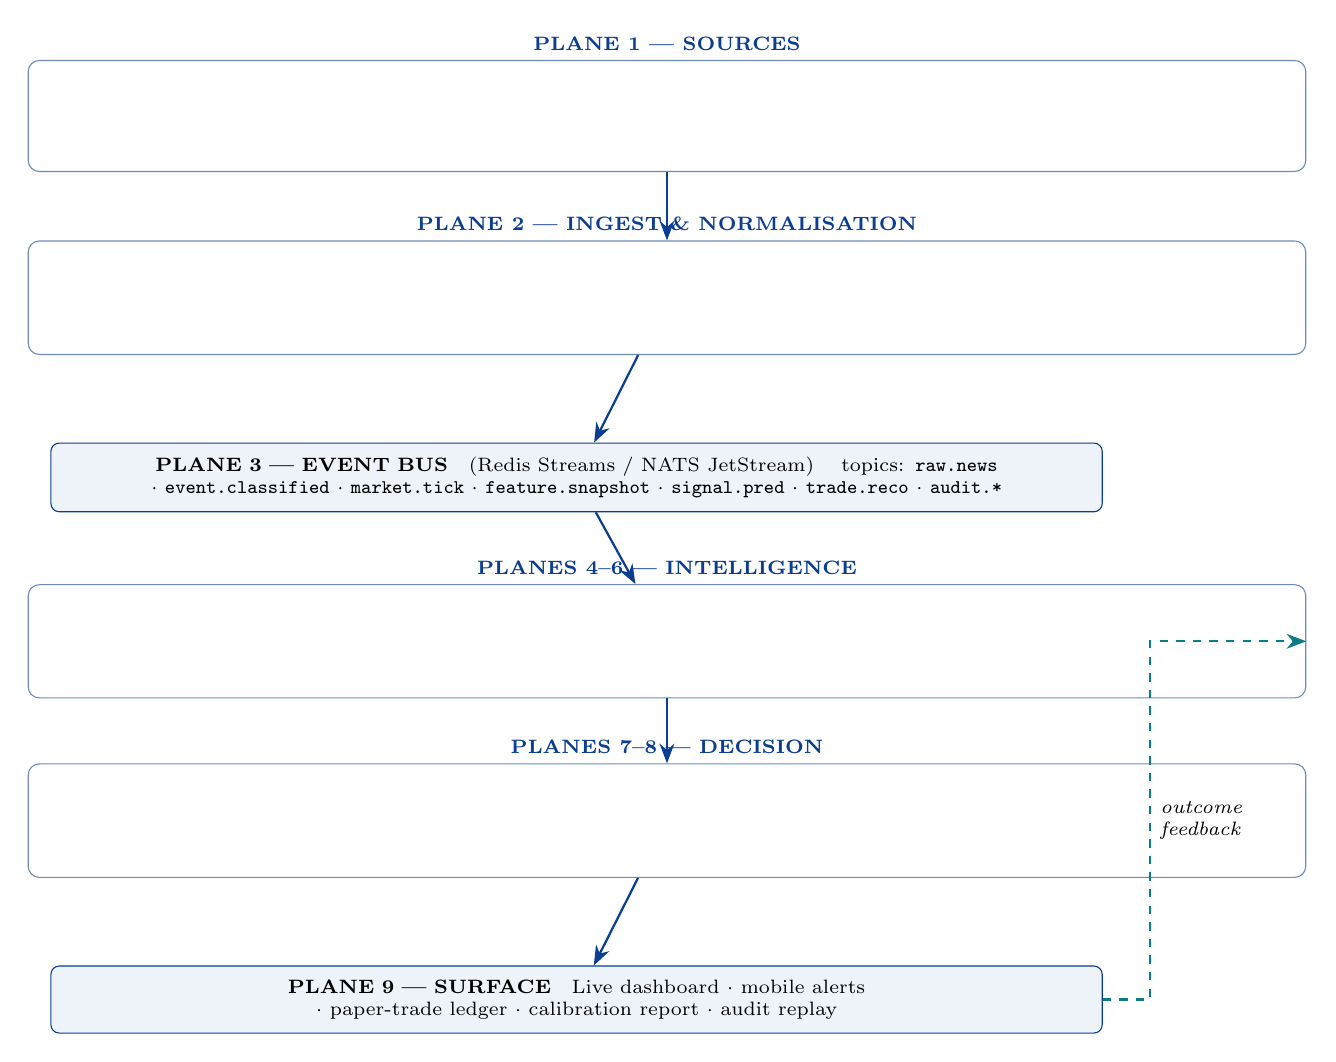
\begin{tikzpicture}[node distance=4mm,every node/.append style={transform shape},scale=1]

% Plane 1 - sources
\node[wide,fill=white] (n1) {Social \& short-form feeds};
\node[wide,fill=white,right=of n1] (n2) {Wires, RSS, gov / central-bank releases};
\node[wide,fill=white,right=of n2] (n3) {Economic calendar + consensus};
\node[wide,fill=white,right=of n3] (n4) {Market \& option-chain feed};
\node[lay,fit=(n1)(n2)(n3)(n4),label={[font=\scriptsize\bfseries,color=msblue]above:PLANE 1 --- SOURCES}] (P1) {};

% Plane 2 - ingest
\node[wide,below=16mm of n1.south west,anchor=north west] (i1) {Collectors\\(async, per-source)};
\node[wide,right=of i1] (i2) {Normaliser\\+ publish-time resolver};
\node[wide,right=of i2] (i3) {Dedup: SimHash\\+ embedding ANN};
\node[wide,right=of i3] (i4) {Tick handler\\+ candle builder};
\node[lay,fit=(i1)(i2)(i3)(i4),label={[font=\scriptsize\bfseries,color=msblue]above:PLANE 2 --- INGEST \& NORMALISATION}] (P2) {};

% Plane 3 - bus
\node[wide,below=14mm of i1.south west,anchor=north west,text width=13.0cm] (bus)
 {\textbf{PLANE 3 --- EVENT BUS} \; (Redis Streams / NATS JetStream) \;\; topics:
  \texttt{raw.news} $\cdot$ \texttt{event.classified} $\cdot$ \texttt{market.tick} $\cdot$
  \texttt{feature.snapshot} $\cdot$ \texttt{signal.pred} $\cdot$ \texttt{trade.reco} $\cdot$ \texttt{audit.*}};

% Plane 4-6
\node[wide,below=12mm of bus.south west,anchor=north west] (e1) {Event Detection\\(2-tier NLP)};
\node[wide,right=of e1] (e2) {Impact Scoring\\(Bayesian priors)};
\node[wide,right=of e2] (e3) {Feature Store\\(online + offline)};
\node[wide,right=of e3] (e4) {Prediction\\Ensemble};
\node[lay,fit=(e1)(e2)(e3)(e4),label={[font=\scriptsize\bfseries,color=msblue]above:PLANES 4--6 --- INTELLIGENCE}] (P4) {};

% Plane 7-8
\node[wide,below=14mm of e1.south west,anchor=north west] (o1) {Candle Projector\\(quantile fan)};
\node[wide,right=of o1] (o2) {IV Surface\\+ Greeks};
\node[wide,right=of o2] (o3) {Structure Selector\\+ Sizing};
\node[wide,right=of o3] (o4) {Risk Gate\\+ Kill switches};
\node[lay,fit=(o1)(o2)(o3)(o4),label={[font=\scriptsize\bfseries,color=msblue]above:PLANES 7--8 --- DECISION}] (P7) {};

% Plane 9
\node[wide,below=14mm of o1.south west,anchor=north west,text width=13.0cm] (ui)
 {\textbf{PLANE 9 --- SURFACE} \; Live dashboard $\cdot$ mobile alerts $\cdot$
  paper-trade ledger $\cdot$ calibration report $\cdot$ audit replay};

\draw[ar] (P1) -- (P2);
\draw[ar] (P2) -- (bus);
\draw[ar] (bus) -- (P4);
\draw[ar] (P4) -- (P7);
\draw[ar] (P7) -- (ui);
\draw[arg] (ui.east) -- ++(0.6,0) |- node[pos=0.25,right,font=\scriptsize\itshape,text width=1.6cm]{outcome feedback} (P4.east);
\end{tikzpicture}
\end{center}

\section{Plane responsibilities and contracts}

\begin{longtable}{@{}p{2.2cm}p{5.4cm}p{6.8cm}@{}}
\toprule
\textbf{Plane} & \textbf{Owns} & \textbf{Hard contract it must honour}\\
\midrule
\endhead
1 Sources & Nothing (external) & Every item must carry an original publish
timestamp or be flagged \texttt{ts\_uncertain}.\\
2 Ingest & Collectors, normaliser, dedup, candle builder & Emits only immutable,
schema-versioned records. Never mutates history. Idempotent on replay.\\
3 Bus & Ordering, durability, replay & At-least-once delivery, consumer groups,
7-day retention hot, cold archive to Parquet.\\
4 Event & Taxonomy classification, entity extraction, novelty, credibility &
Emits an \texttt{Event} with class, severity, confidence, entities, novelty and
credibility. Never emits a trade opinion.\\
5 Impact & Historical conditional response distributions & Emits a distribution
over index returns per horizon, plus sample size and confidence interval.
Refuses to answer when $n < 8$.\\
6 Features & Online and offline feature computation & \emph{Identical code path}
for training and serving. Every feature carries an as-of timestamp.\\
7 Prediction & Direction, magnitude, volatility, quantiles & Outputs calibrated
probabilities and conformal intervals. Must attach model version and feature
hash.\\
8 Decision & Structure choice, sizing, risk & May veto anything. Owns all
kill-switches. Writes an immutable decision record with full reasoning.\\
9 Surface & Presentation, alerting, ledger & Read-only with respect to trading
state; may not influence decisions.\\
\bottomrule
\end{longtable}

\section{Two speed lanes}

A recurring failure in such systems is trying to make everything fast. Instead,
split explicitly:

\begin{longtable}{@{}p{3.2cm}p{5.4cm}p{5.8cm}@{}}
\toprule
& \textbf{Hot lane (reflex)} & \textbf{Cold lane (deliberation)}\\
\midrule
Latency budget & Under 400 ms end to end & 1--60 seconds\\
Triggered by & Breaking event, price shock, scheduled release & Every event,
plus a 5-second heartbeat\\
Models used & Quantised, pre-warmed, small; rules and lookups & Full ensemble,
LLM reasoning, cross-source confirmation, Monte Carlo\\
Output & Provisional alert with wide intervals & Full recommendation with
structure and sizing\\
Can it place an order? & No. Never. & Yes (once Tier T4 is reached)\\
Rationale & Speed without confirmation is how you trade a fake headline &
Confirmation without speed misses the move; two lanes get both\\
\bottomrule
\end{longtable}

\begin{keybox}[title={The two-lane rule}]
The hot lane says \emph{``something is happening, widen your risk''}.
The cold lane says \emph{``here is the trade''}. Conflating them is the design
error that turns a research system into an account-destroying machine.
\end{keybox}

\section{Technology choices with justification}

\begin{longtable}{@{}p{3.0cm}p{4.0cm}p{7.4cm}@{}}
\toprule
\textbf{Layer} & \textbf{Choice} & \textbf{Why this, not the alternative}\\
\midrule
Language (services) & Python 3.12 + \texttt{asyncio} + \texttt{uvloop} &
Ecosystem for ML is decisive. \texttt{uvloop} closes most of the gap for I/O
bound work. Rewrite only the proven hot path later, if profiling demands it.\\
Language (hot path, later) & Rust (via PyO3) & Only for the tick handler and
candle builder if p99 exceeds budget. Do not start here.\\
API & FastAPI & Async, typed, automatic OpenAPI, WebSocket support.\\
Event bus & Redis Streams (v1) $\to$ NATS JetStream (v2) & Redis Streams gives
consumer groups and replay with zero extra infrastructure since Redis is
already needed for the online feature store. Kafka is operationally heavy for a
single-node start; NATS is the low-latency upgrade path.\\
Time-series store & PostgreSQL + TimescaleDB & Hypertables, continuous
aggregates for candle roll-ups, compression, and plain SQL. Avoids a separate
query language.\\
Research store & Parquet on local NVMe + DuckDB & Backtests are analytical
scans, not point lookups. DuckDB over Parquet is dramatically faster and
simpler than querying the OLTP database.\\
Online feature store & Redis (hashes + sorted sets) & Sub-millisecond reads,
TTL semantics match feature freshness.\\
Vector search & FAISS or \texttt{pgvector} & Deduplication and
nearest-historical-event retrieval. \texttt{pgvector} first for operational
simplicity.\\
Model training & PyTorch, LightGBM, scikit-learn & LightGBM is the baseline that
usually wins on tabular features; PyTorch for sequence and distribution models.\\
Model serving & ONNX Runtime & Removes Python overhead at inference; consistent
across CPU and GPU; batch-1 latency is what matters here.\\
NLP models & A financial-domain encoder for sentiment/classification, a
multilingual encoder for global sources, plus an LLM in the cold lane only &
Encoders are fast and cheap; the LLM is reserved for reasoning where its latency
is affordable.\\
Orchestration & Prefect or Dagster & Nightly retrains, data quality checks,
backfills. Airflow is heavier than needed.\\
Experiment tracking & MLflow & Model registry plus metric lineage; the registry
is what production reads from.\\
Frontend & React + TypeScript + a lightweight charting library & TradingView's
free charting library is acceptable for candles; the fan-chart overlay is custom
canvas work.\\
Transport to UI & WebSocket with binary framing (MessagePack) & JSON at 1 Hz per
instrument is fine; at tick rate it is not.\\
Containerisation & Docker Compose (v1) $\to$ Kubernetes (only at multi-user) &
Kubernetes before Tier~T5 is pure overhead.\\
Monitoring & Prometheus + Grafana + structured JSON logs + OpenTelemetry traces
& A trace ID must flow from the news item all the way to the recommendation.\\
\bottomrule
\end{longtable}

\begin{warnbox}[title={Deployment location matters more than framework choice}]
Co-locate compute in the same cloud region as your broker/data endpoints
(for NSE-facing infrastructure this generally means a Mumbai region). A poor
region choice adds more latency than every micro-optimisation in this document
combined.
\end{warnbox}

\section{Failure domains and degradation}

\begin{longtable}{@{}p{3.8cm}p{4.2cm}p{6.4cm}@{}}
\toprule
\textbf{Failure} & \textbf{Detection} & \textbf{Degraded behaviour}\\
\midrule
News source down & No heartbeat for 90 s & Mark source stale; reduce credibility
weight of single-source events; continue on market-only features.\\
Market feed gap & Sequence gap or 3 s silence during market hours & Halt all new
signals immediately. Flatten open paper positions at last known price. Alert.\\
Model server unhealthy & p99 latency or error rate breach & Fall back to the
rules-only baseline model, flag every output as \texttt{DEGRADED}, forbid
auto-execution.\\
Clock drift $>$ 50 ms & NTP monitor & Refuse to emit signals. Time integrity is
non-negotiable for point-in-time correctness.\\
Redis unavailable & Connection error & Hot lane stops; cold lane continues from
TimescaleDB with a wider latency SLO.\\
Contradictory events & Two opposing high-severity events within 60 s & Emit
\texttt{CONFLICT}; suppress all directional signals; volatility signals only.\\
\bottomrule
\end{longtable}

% =====================================================================
\chapter{Data Layer}
% =====================================================================

\section{Source catalogue}

Sources are tiered by credibility. Credibility is a numeric weight used later in
impact scoring, not a binary trust decision.

\begin{longtable}{@{}p{4.0cm}p{2.3cm}p{2.3cm}p{5.6cm}@{}}
\toprule
\textbf{Source class} & \textbf{Credibility $c$} & \textbf{Typical lag} &
\textbf{Role}\\
\midrule
Central bank / regulator official release & 1.00 & 0--2 s & Ground truth for
policy events. Scrape the official page directly, not a news summary of it.\\
Exchange notices & 1.00 & 0--5 s & Halts, bans, margin changes.\\
Major international wires & 0.90 & 1--10 s & Primary breaking coverage.\\
Verified official accounts of heads of state / ministries & 0.85 & 0--3 s &
Highest-impact, highest-noise. Requires source-specific handling.\\
Tier-1 national business media & 0.75 & 30--180 s & Confirmation, colour.\\
Aggregator APIs & 0.60 & 60--600 s & Breadth, not speed.\\
Anonymous social accounts & 0.15--0.35 & 0--5 s & Early warning only. May
\emph{never} independently trigger a directional trade.\\
Forums and community feeds & 0.10 & Variable & Sentiment aggregate only.\\
\bottomrule
\end{longtable}

\subsection{Market data}

\begin{longtable}{@{}p{4.0cm}p{3.2cm}p{7.0cm}@{}}
\toprule
\textbf{Stream} & \textbf{Frequency} & \textbf{Use}\\
\midrule
Index spot (Nifty, Bank Nifty, Fin Nifty) & Tick or 1/s & Base price series,
candle construction.\\
Index futures & Tick or 1/s & Basis, and it often leads spot.\\
Full option chain (both indices, near two expiries) & 1--5 s snapshot &
Implied volatility surface, open interest, put-call ratio, max pain,
gamma exposure.\\
India VIX & 1/s & Regime variable, volatility term structure anchor.\\
GIFT/SGX Nifty & Tick & Overnight and pre-open leading indicator.\\
Global futures (US equity index, crude, gold), DXY, USDINR & 1/s or 1-min &
Cross-asset propagation, overnight event pricing.\\
Sector indices & 1/s & Event-to-sector routing.\\
Participant-wise open interest, FII/DII flows & End of day & Positioning
regime features.\\
Corporate actions, expiry calendar, holiday calendar & Static/daily &
Absolutely required to avoid silent backtest corruption.\\
\bottomrule
\end{longtable}

\section{The candle builder (and why it is subtle)}

Building 1-minute candles from ticks looks trivial and is the most common source
of quiet data corruption. Requirements:

\begin{enumerate}
\item \term{Exchange time, not local time.} Every timestamp normalised to
exchange time with explicit timezone; store as UTC with an exchange-time view.
\item \term{Left-closed, right-open intervals.} A tick at exactly 09:20:00.000
belongs to the 09:20 candle, not 09:19.
\item \term{Explicit gap handling.} If no tick arrives in a minute, emit a
zero-volume candle with $O=H=L=C=$ previous close, flagged \texttt{synthetic}.
Silent omission destroys sequence models.
\item \term{Session boundaries.} Pre-open (09:00--09:15) is a different price
formation mechanism; tag it, never mix it into continuous-session statistics.
\item \term{Late ticks.} A tick arriving after its candle is sealed goes to a
correction log; the candle is versioned, not overwritten in place.
\item \term{Determinism.} Replaying the same tick file must yield a
byte-identical candle file. Enforce this with a test.
\end{enumerate}

\section{Point-in-time discipline}

\begin{keybox}[title={The three timestamps}]
Every record carries three timestamps, always:
\begin{itemize}
\item \texttt{t\_event} --- when the thing happened in the world (publish time).
\item \texttt{t\_ingest} --- when our system first saw it.
\item \texttt{t\_available} --- when it became usable for a decision (after
dedup, classification and feature computation).
\end{itemize}
\textbf{Backtests may only use data where \texttt{t\_available} $\le$ the
decision time.} A feature computed from \texttt{t\_event} alone is look-ahead
bias wearing a disguise.
\end{keybox}

Revised data (an economic figure corrected an hour later, an option chain
snapshot re-published) is stored as a new row with a validity interval, never as
an update. The research layer always reads ``the value as known at time $t$''.

\section{Storage layout}

\begin{lstlisting}[language=SQL,caption={Core TimescaleDB schema (abridged)}]
-- Ticks: hypertable partitioned by day, compressed after 7 days
CREATE TABLE tick (
  ts            TIMESTAMPTZ   NOT NULL,
  instrument_id INT           NOT NULL,
  ltp           NUMERIC(12,2) NOT NULL,
  qty           INT,
  bid           NUMERIC(12,2), ask NUMERIC(12,2),
  bid_qty       INT,           ask_qty INT,
  oi            BIGINT,
  seq           BIGINT        NOT NULL,   -- gap detection
  src           SMALLINT      NOT NULL
);
SELECT create_hypertable('tick','ts', chunk_time_interval => INTERVAL '1 day');

-- Candles: one row per (instrument, timeframe, bucket)
CREATE TABLE candle (
  ts TIMESTAMPTZ NOT NULL, instrument_id INT NOT NULL, tf SMALLINT NOT NULL,
  o NUMERIC(12,2), h NUMERIC(12,2), l NUMERIC(12,2), c NUMERIC(12,2),
  v BIGINT, oi BIGINT, trades INT,
  vwap NUMERIC(12,2), synthetic BOOLEAN DEFAULT FALSE, version SMALLINT DEFAULT 1,
  PRIMARY KEY (instrument_id, tf, ts, version)
);

-- Option chain snapshots
CREATE TABLE option_snap (
  ts TIMESTAMPTZ NOT NULL, underlying_id INT, expiry DATE,
  strike NUMERIC(10,2), opt_type CHAR(2),
  ltp NUMERIC(10,2), bid NUMERIC(10,2), ask NUMERIC(10,2),
  volume BIGINT, oi BIGINT, oi_change BIGINT,
  iv NUMERIC(6,3), delta NUMERIC(6,4), gamma NUMERIC(10,8),
  theta NUMERIC(8,4), vega NUMERIC(8,4), rho NUMERIC(8,4),
  spot NUMERIC(12,2)
);

-- News / event store: append-only, point-in-time
CREATE TABLE news_raw (
  id UUID PRIMARY KEY,
  t_event TIMESTAMPTZ, t_ingest TIMESTAMPTZ NOT NULL, ts_uncertain BOOLEAN,
  source_id INT NOT NULL, url TEXT, lang CHAR(3),
  headline TEXT, body TEXT, content_hash BYTEA, simhash BIGINT,
  embedding vector(768)
);

CREATE TABLE event_classified (
  id UUID PRIMARY KEY, news_id UUID REFERENCES news_raw(id),
  t_available TIMESTAMPTZ NOT NULL,
  event_class TEXT NOT NULL, subclass TEXT,
  severity NUMERIC(3,1), confidence NUMERIC(4,3),
  novelty NUMERIC(4,3), credibility NUMERIC(4,3),
  entities JSONB, geo JSONB, surprise NUMERIC(8,4),
  model_version TEXT NOT NULL
);
\end{lstlisting}

\begin{longtable}{@{}p{3.4cm}p{3.0cm}p{7.8cm}@{}}
\toprule
\textbf{Data} & \textbf{Hot store} & \textbf{Cold store / research}\\
\midrule
Ticks & TimescaleDB 7 days & Daily Parquet, partitioned
\texttt{/date=/instrument=}\\
Candles & TimescaleDB, all & Parquet mirror for DuckDB scans\\
Option chain & TimescaleDB 30 days & Parquet, partitioned by date and expiry\\
News \& events & PostgreSQL, all & Parquet + embeddings index\\
Features & Redis (TTL 15 min) & Parquet feature snapshots per decision\\
Decisions \& outcomes & PostgreSQL, all & Never deleted. This is the audit
spine.\\
\bottomrule
\end{longtable}

\section{Data quality gates (run continuously)}

\begin{longtable}{@{}p{4.4cm}p{4.0cm}p{6.0cm}@{}}
\toprule
\textbf{Check} & \textbf{Threshold} & \textbf{Action on breach}\\
\midrule
Tick sequence gaps & any gap & Log, backfill from broker history, mark affected
minute untrusted.\\
Candle count per session & exactly 375 for continuous session & Block research
jobs on that day until resolved.\\
Option chain completeness & $\ge$ 95\% of expected strikes & Do not compute
surface; mark surface stale.\\
Implied volatility sanity & $0.03 < \sigma < 3.0$, no-arbitrage monotonic in
strike & Reject the quote, use surface fit instead.\\
Put-call parity deviation & beyond spread-implied bound & Flag stale quote; do
not trade that strike.\\
News timestamp sanity & \texttt{t\_event} $\le$ \texttt{t\_ingest} and within 7
days & Set \texttt{ts\_uncertain}, exclude from latency-sensitive research.\\
Duplicate rate & $<$ 3\% post-dedup & Retune dedup thresholds.\\
Feature null rate & $<$ 1\% per feature per day & Block model training.\\
Train/serve skew & feature distribution PSI $< 0.2$ & Alert; investigate before
next retrain.\\
\bottomrule
\end{longtable}

% =====================================================================
\chapter{Event Detection Engine}
\label{ch:event}
% =====================================================================

\section{The funnel}

Roughly 500{,}000 items per day may enter the pipeline. Perhaps 40 are worth a
model's attention and 3 are worth a trade. The engine is therefore a funnel with
increasing cost per stage.

\begin{center}
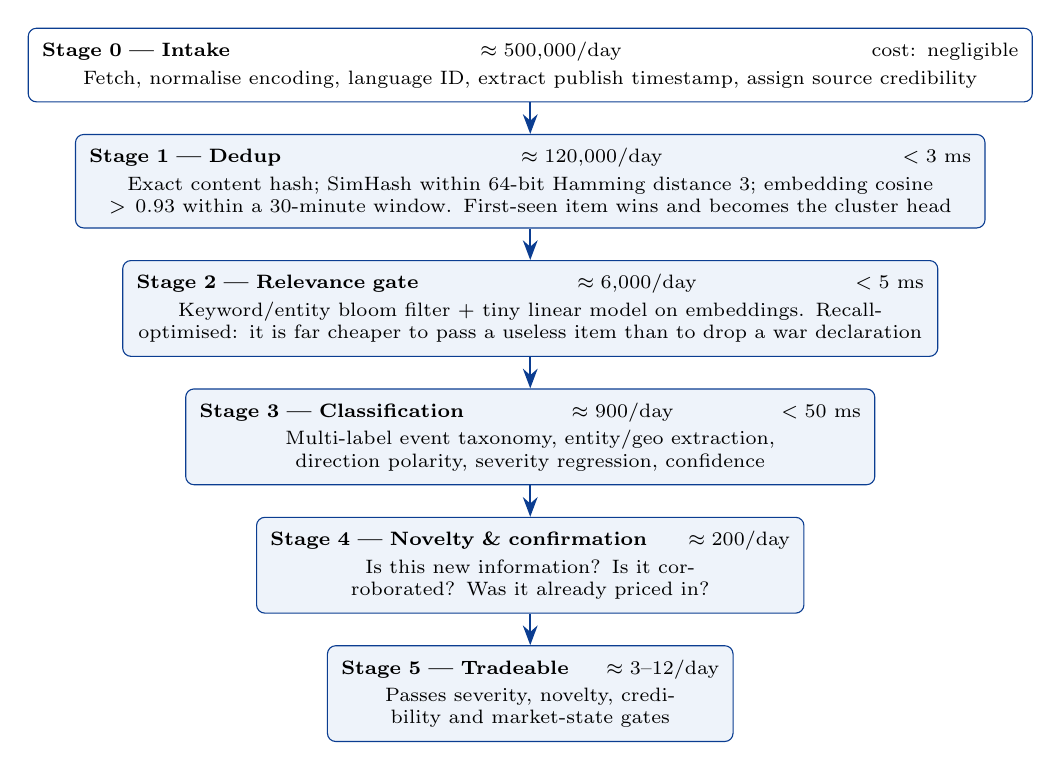
\begin{tikzpicture}[node distance=4mm]
\node[wide,text width=12.4cm,fill=white] (s0) {\textbf{Stage 0 --- Intake} \hfill $\approx 500{,}000$/day \hfill cost: negligible\\[2pt]
\scriptsize Fetch, normalise encoding, language ID, extract publish timestamp, assign source credibility};
\node[wide,text width=11.2cm,below=of s0] (s1) {\textbf{Stage 1 --- Dedup} \hfill $\approx 120{,}000$/day \hfill $<3$ ms\\[2pt]
\scriptsize Exact content hash; SimHash within 64-bit Hamming distance 3; embedding cosine $>0.93$ within a 30-minute window. First-seen item wins and becomes the cluster head};
\node[wide,text width=10.0cm,below=of s1] (s2) {\textbf{Stage 2 --- Relevance gate} \hfill $\approx 6{,}000$/day \hfill $<5$ ms\\[2pt]
\scriptsize Keyword/entity bloom filter + tiny linear model on embeddings. Recall-optimised: it is far cheaper to pass a useless item than to drop a war declaration};
\node[wide,text width=8.4cm,below=of s2] (s3) {\textbf{Stage 3 --- Classification} \hfill $\approx 900$/day \hfill $<50$ ms\\[2pt]
\scriptsize Multi-label event taxonomy, entity/geo extraction, direction polarity, severity regression, confidence};
\node[wide,text width=6.6cm,below=of s3] (s4) {\textbf{Stage 4 --- Novelty \& confirmation} \hfill $\approx 200$/day\\[2pt]
\scriptsize Is this new information? Is it corroborated? Was it already priced in?};
\node[wide,text width=4.8cm,below=of s4] (s5) {\textbf{Stage 5 --- Tradeable} \hfill $\approx 3$--$12$/day\\[2pt]
\scriptsize Passes severity, novelty, credibility and market-state gates};
\draw[ar](s0)--(s1); \draw[ar](s1)--(s2); \draw[ar](s2)--(s3); \draw[ar](s3)--(s4); \draw[ar](s4)--(s5);
\end{tikzpicture}
\end{center}

\begin{keybox}[title={Asymmetric error policy}]
Stages 0--2 are tuned for \textbf{recall} (never lose a real event). Stages 3--5
are tuned for \textbf{precision} (never trade a non-event). Mixing these
objectives in one model is the classic mistake.
\end{keybox}

\section{Event taxonomy}

The taxonomy is the backbone of the entire system: impact priors, features,
model conditioning and post-trade attribution are all keyed on it. It must be
designed once, carefully, and versioned.

\begin{longtable}{@{}p{3.3cm}p{4.4cm}p{2.1cm}p{4.4cm}@{}}
\toprule
\textbf{Family} & \textbf{Classes (examples)} & \textbf{Typical\newline severity}
& \textbf{Primary Indian transmission channel}\\
\midrule
\endhead
Monetary policy & rate decision, stance change, liquidity measure, unscheduled
action, minutes/commentary & 6--10 & Bank Nifty directly; rate-sensitive
sectors; currency\\
Macro release & inflation, growth, employment, trade balance, industrial output,
fiscal data & 4--8 & Broad index via surprise vs consensus\\
Geopolitical & military action, escalation rhetoric, territorial incident,
sanctions, treaty, coup & 3--10 & Risk premium, crude, currency, gold; defence
and oil-marketing sectors\\
Trade \& tariffs & tariff announcement, export ban, supply-chain restriction &
4--9 & Export sectors (IT, pharma, chemicals, textiles)\\
Energy & production quota change, supply disruption, strategic reserve action,
pipeline/refinery incident & 4--9 & Crude to inflation to rates; paint,
aviation, oil marketing, tyres\\
Domestic policy & budget item, regulatory change, sector reform, tax change,
subsidy & 3--9 & Sector-specific, occasionally index-wide\\
Corporate/market structure & index rebalancing, large block deal, big listing,
margin/regulatory change & 3--7 & Flow-driven, highly mechanical, often the most
predictable class\\
Flows \& positioning & foreign flow reversal, large open-interest shift,
expiry-day pinning & 3--6 & Mechanical, intraday, exploitable\\
Disaster \& health & natural disaster, epidemic, major infrastructure failure &
2--9 & Insurance, infrastructure, supply chains\\
Political & election result, coalition change, major resignation, scandal &
3--10 & Broad risk premium; extremely high variance\\
Noise / non-event & opinion, analysis, repetition, speculation & 0--2 &
\textbf{Explicit class} --- the model must learn to say ``nothing here''\\
\bottomrule
\end{longtable}

Each classified event carries the following fields.

\begin{longtable}{@{}p{3.2cm}p{2.4cm}p{9.0cm}@{}}
\toprule
\textbf{Field} & \textbf{Type} & \textbf{Meaning and how it is produced}\\
\midrule
\texttt{class}, \texttt{subclass} & enum & Multi-label transformer classifier.\\
\texttt{polarity} & $[-1,1]$ & Risk-off ($-1$) to risk-on ($+1$) for Indian
equities specifically --- \emph{not} generic sentiment. A rate cut is negative
sentiment about growth but positive polarity for equities.\\
\texttt{severity} & $[0,10]$ & Regression head trained on human-labelled
anchors; described in Section~\ref{sec:severity}.\\
\texttt{confidence} & $[0,1]$ & Classifier probability, temperature-calibrated.\\
\texttt{entities} & list & Countries, institutions, commodities, companies,
sectors --- linked to a canonical knowledge graph, not free text.\\
\texttt{geo} & list & Location plus a distance/exposure weight to India.\\
\texttt{novelty} & $[0,1]$ & Section~\ref{sec:novelty}.\\
\texttt{credibility} & $[0,1]$ & Source weight, boosted by corroboration.\\
\texttt{surprise} & $\mathbb{R}$ & For scheduled events: $(\text{actual} -
\text{consensus})/\sigma_{\text{consensus}}$. Null otherwise.\\
\texttt{expected} & bool & Was this event on the calendar? Scheduled and
unscheduled events behave completely differently.\\
\bottomrule
\end{longtable}

\section{Severity: how to make it real and not arbitrary}
\label{sec:severity}

A hand-written severity table will not survive contact with reality. Build
severity in three passes:

\begin{enumerate}
\item \term{Anchor set.} Hand-label 400--600 historical headlines on a 0--10
scale using written rubrics with concrete anchors (10 = existential shock;
7 = major unexpected policy shift; 4 = meaningful but priced; 1 = commentary).
Two labellers, measure inter-annotator agreement, resolve disagreements.
\item \term{Supervised head.} Train a regression head on the encoder to predict
the anchor scores.
\item \term{Empirical recalibration.} This is the step everyone skips: regress
the predicted severity against the \emph{realised} absolute abnormal move of
Nifty in the following 30 minutes across all historical events. Then remap
severity so that it is monotonic in realised impact. Severity becomes an
\emph{empirically grounded} quantity rather than an opinion.
\end{enumerate}

\[
\text{severity}^{\text{cal}} = F^{-1}_{|r_{30}|}\!\left(
\hat{F}_{\text{sev}}\big(\text{severity}^{\text{raw}}\big)\right)
\]
where $\hat F_{\text{sev}}$ is the empirical CDF of raw severity and
$F_{|r_{30}|}$ the empirical CDF of absolute 30-minute abnormal returns.

\section{Novelty: is this actually new information?}
\label{sec:novelty}

The most expensive mistake is trading a re-report of something already priced.
Novelty combines four signals:

\begin{align*}
\text{novelty} \;=\;\;& w_1 \underbrace{\big(1-\max_j \cos(e, e_j)\big)}_{\text{semantic distance to last 6 h}}
\;+\; w_2 \underbrace{\mathbb{1}[\text{first mention in cluster}]}_{\text{primacy}} \\[5pt]
+\;& w_3 \underbrace{(1 - \rho_{\text{cal}})}_{\text{not on calendar}}
\;+\; w_4 \underbrace{\big(1 - |\hat r_{\text{pre}}| / \sigma_{5}\big)}_{\text{market has not already moved}}
\end{align*}

The fourth term is the most underrated: if the index has already moved two
standard deviations in the five minutes \emph{before} our detection, the
information is in the price and the opportunity has passed. In that case the
system should consider a \emph{fade} strategy or, more usually, no trade at all.

\section{Confirmation and the fake-news defence}

\begin{longtable}{@{}p{3.4cm}p{5.2cm}p{5.8cm}@{}}
\toprule
\textbf{Rule} & \textbf{Condition} & \textbf{Consequence}\\
\midrule
Single low-credibility source & $c < 0.5$, no corroboration & Hot-lane alert
only. No directional signal. Volatility-widening only.\\
Corroboration window & Second independent source with $c \ge 0.75$ within 120 s
& Credibility upgraded; directional signal permitted.\\
Official confirmation & Primary source (regulator, central bank, exchange,
official channel) & Full weight immediately.\\
Contradiction & An equally credible source contradicts within 5 min & Emit
\texttt{RETRACTION}; immediately close any position opened on that event and
mark the event poisoned.\\
Extreme severity gate & severity $\ge 9$ & Requires \textbf{two} independent
sources with $c \ge 0.8$ regardless of speed. The most extreme headlines are the
most likely to be fake.\\
Market disagreement & Signal says down, but index, futures and currency all move
up within 30 s & Suppress. The market is a better classifier than we are.\\
\bottomrule
\end{longtable}

\begin{warnbox}[title={The AP-hack test}]
Before going live, run this test: inject a synthetic, highly credible-looking
but false catastrophic headline from a single medium-credibility source into a
replay. \textbf{The system must not produce a directional trade.} If it does,
the confirmation logic is wrong. Repeat this test in CI forever.
\end{warnbox}

\section{Entity-to-instrument routing}

An event mentioning ``crude supply disruption'' must mechanically become an
exposure vector. Maintain a knowledge graph:

\begin{lstlisting}[language=Python,caption={Exposure routing (conceptual)}]
# knowledge graph edge: (entity) --affects--> (factor) --loads_on--> (instrument)
EXPOSURE = {
    "crude_oil": {"NIFTY": -0.25, "BANKNIFTY": -0.15,
                  "sector:OIL_MKTG": -0.80, "sector:AVIATION": -0.70,
                  "sector:PAINTS": -0.55, "sector:UPSTREAM": +0.60},
    "usd_inr_up": {"NIFTY": -0.20, "sector:IT": +0.65, "sector:PHARMA": +0.40},
    "rbi_rate_cut": {"BANKNIFTY": +0.70, "NIFTY": +0.45,
                     "sector:REALTY": +0.75, "sector:AUTO": +0.55},
}
# Beta values are ESTIMATED FROM HISTORY (rolling regression), never hand-typed
# in production. The dict above is only the bootstrap prior for cold start.
\end{lstlisting}

\begin{keybox}[title={Rule}]
Hand-written coefficients are acceptable only as a cold-start prior. Every
coefficient must be replaced by a rolling empirical estimate with a confidence
interval as soon as sufficient history exists. The system must be able to answer
``how do you know?'' with a number and a sample size.
\end{keybox}

% =====================================================================
\chapter{Impact Scoring Engine}
\label{ch:impact}
% =====================================================================

\section{What impact scoring actually is}

The original design computes ``Nifty will drop 1.5\%''. That is a point estimate
with no error bar, and it is the root cause of over-sizing. The correct object
is a \term{conditional predictive distribution}:

\[
P\big(r_{t \to t+h} \;\big|\; \text{event class } c,\ \text{severity } s,\
\text{surprise } z,\ \text{market state } m\big)
\]

produced primarily from historical evidence, and used as a \emph{prior} that the
ML models in Chapter~\ref{ch:ml} then update with live microstructure.

\section{Building the impact library: event study methodology}

For every historical event of class $c$:

\begin{enumerate}
\item Define the event time $t_0$ precisely (publish timestamp, exchange time).
\item Compute the \term{abnormal return} over horizon $h$: subtract the expected
return given the market's normal behaviour at that time of day and volatility
regime,
\[
AR_{h} = r_{t_0 \to t_0+h} - \hat{\mathbb{E}}\!\left[r_{h} \mid
\text{time-of-day}, \sigma_{\text{regime}}, \text{day-type}\right].
\]
Time-of-day normalisation matters enormously in Indian intraday data: the
volatility profile is strongly U-shaped, so a raw 0.3\% move at 09:20 is
ordinary while the same move at 13:30 is extreme.
\item Compute a matched \term{control distribution}: sample non-event windows
with the same time-of-day and volatility regime.
\item Record: $AR_h$ for $h \in \{1,5,15,30,60\}$ minutes, realised volatility
ratio, implied volatility change, maximum favourable and adverse excursion,
volume ratio, and time-to-peak.
\item Test significance against the control distribution with a bootstrap, not a
normal approximation (intraday returns are fat-tailed).
\end{enumerate}

\begin{longtable}{@{}p{4.0cm}p{10.6cm}@{}}
\toprule
\textbf{Stored statistic} & \textbf{Why it matters for trading}\\
\midrule
Median $AR_h$ and quantiles & The realistic expectation and its spread.\\
$P(\text{sign correct})$ & Whether a directional trade is even sensible.\\
Realised-vol ratio $\sigma_{\text{post}}/\sigma_{\text{pre}}$ & Whether to buy
volatility.\\
$\Delta\sigma_{\text{IV}}$ distribution & \textbf{The vega decision.} Determines
whether options get more or less expensive.\\
Max favourable / adverse excursion & Where to put the target and the stop, from
evidence rather than a round number.\\
Time-to-peak & The correct holding period; also determines the horizon to trade.\\
Half-life of the effect & Whether the move persists or mean-reverts.\\
Sample size $n$ & The honesty check.\\
\bottomrule
\end{longtable}

\section{Hierarchical Bayesian shrinkage for rare events}

Most interesting events are rare. With $n=4$ historical instances, the empirical
mean is noise. Use a hierarchical model that shrinks class-level estimates
toward their family-level estimate:

\[
\mu_c \sim \mathcal{N}(\mu_{\text{family}}, \tau^2), \qquad
AR_{c,i} \sim \mathcal{N}(\mu_c \cdot g(s_i), \sigma_c^2)
\]

with posterior mean approximately
\[
\hat\mu_c = \frac{n_c/\sigma_c^2}{n_c/\sigma_c^2 + 1/\tau^2}\,\bar{AR}_c
\;+\; \frac{1/\tau^2}{n_c/\sigma_c^2 + 1/\tau^2}\,\mu_{\text{family}} .
\]

\begin{keybox}[title={Practical consequence}]
With $n_c = 3$, the estimate is dominated by the family prior --- which is
exactly correct behaviour. The engine reports the posterior \emph{and} the
sample size, and the risk gate reduces position size when the posterior variance
is high. Refuse to emit a class-specific impact when $n_c < 8$ and no family
prior exists; fall back to ``unknown event, volatility-only response''.
\end{keybox}

\section{The live scoring formula}

\[
\hat{r}_h \;=\; \underbrace{\hat\mu_{c,h}}_{\text{Bayesian prior}}
\times \underbrace{g(s)}_{\text{severity}}
\times \underbrace{\nu}_{\text{novelty}}
\times \underbrace{c_{\text{cred}}}_{\text{credibility}}
\times \underbrace{\kappa(m)}_{\text{regime}}
\times \underbrace{\lambda(\tau)}_{\text{time-of-day}}
\times \underbrace{(1-\pi)}_{\text{already-priced discount}}
\]

\begin{longtable}{@{}p{2.2cm}p{4.0cm}p{8.4cm}@{}}
\toprule
\textbf{Term} & \textbf{Form} & \textbf{Notes}\\
\midrule
$g(s)$ & $\left(s/5\right)^{\gamma}$, $\gamma \approx 1.4$ fitted &
Impact is convex in severity: a 9 is much more than twice a 4.5.\\
$\nu$ & novelty score & Old news gets multiplied toward zero.\\
$c_{\text{cred}}$ & credibility & Unconfirmed rumour is heavily discounted.\\
$\kappa(m)$ & regime multiplier & Same event has larger impact in a
high-volatility, low-liquidity regime. Fitted per regime cluster.\\
$\lambda(\tau)$ & time-of-day multiplier & U-shaped; also handles the special
cases of the opening 15 minutes, the pre-close and expiry-day afternoons.\\
$\pi$ & $\min\!\big(1, |r_{\text{pre}}| / |\hat\mu_{c,h}|\big)$ &
If the market has already made the expected move before we act, the remaining
opportunity is gone. \textbf{This term is what prevents chasing.}\\
\bottomrule
\end{longtable}

The output is not a scalar but a triple: $(\hat r_h,\ \text{quantiles},\
n_{\text{eff}})$ for each horizon $h$, plus a separate volatility forecast
$(\hat\sigma_{\text{post}}/\sigma_{\text{pre}},\ \widehat{\Delta\sigma_{IV}})$.

\section{Cross-asset propagation}

When an event occurs outside Indian market hours, or affects a foreign asset
first, the impact reaches Nifty through a measurable chain. Estimate the chain
empirically with lagged regressions and store the transfer coefficients:

\begin{longtable}{@{}p{3.6cm}p{3.2cm}p{7.8cm}@{}}
\toprule
\textbf{Channel} & \textbf{Typical lag} & \textbf{Modelling note}\\
\midrule
GIFT/SGX Nifty to Nifty spot & Near-instant during overlap; sets the gap when
Indian market is shut & The single most useful overnight variable.\\
US equity futures to Indian open & Overnight & Estimate a gap model:
$r_{\text{gap}} = \alpha + \beta\, r_{\text{US futures}} + \ldots$\\
Crude to Nifty & Minutes to hours & Asymmetric: sharp spikes transmit faster
than slow drifts.\\
USD/INR to Nifty & Minutes & Bidirectional causality; use a vector
autoregression, not a simple regression.\\
US Treasury yields to Bank Nifty & Hours & Slower; more relevant to the next
session.\\
Asian indices to Nifty intraday & Minutes & Useful during the 09:15--12:00
window.\\
\bottomrule
\end{longtable}

\begin{keybox}[title={The overnight opportunity}]
Roughly half of the total price change in Indian indices arrives as overnight
gaps. Most retail systems ignore this because they only look at intraday
candles. A well-calibrated \term{gap forecaster} driven by overnight global
events is arguably an easier and more profitable first product than intraday
prediction --- and it needs no low-latency infrastructure at all. Consider
shipping it first (see Phase~4 in the roadmap).
\end{keybox}

% =====================================================================
\chapter{Feature Store and Feature Catalogue}
\label{ch:features}
% =====================================================================

\section{Why a feature store and not a script}

The most common cause of a backtest that works and a live system that does not
is \term{train/serve skew}: the offline feature was computed differently from
the online one. The rule is absolute.

\begin{keybox}[title={One definition, two materialisations}]
A feature is defined \emph{once}, in one function, with an explicit dependency
list and an as-of timestamp. The offline path runs it over Parquet history; the
online path runs the same function over Redis state. A CI test replays a live
day offline and asserts every feature matches to within floating-point
tolerance. If it does not match, the build fails.
\end{keybox}

\begin{lstlisting}[language=Python,caption={Feature definition pattern}]
@feature(name="ofi_60s", version=3, deps=["book.bid","book.ask"],
         window="60s", ttl="5s", fill="ffill_max_2")
def order_flow_imbalance(book: BookWindow) -> float:
    """Signed order-flow imbalance over the trailing 60 seconds.
    Point-in-time safe: reads only data with ts <= as_of."""
    ...

# Offline: engine.materialise(ofi_60s, start, end) -> Parquet column
# Online : engine.serve(ofi_60s, as_of=now)        -> float from Redis
# CI     : assert_offline_online_parity(ofi_60s, sample_day)
\end{lstlisting}

\section{Feature catalogue}

\subsection{Group A --- Price and trend (the baseline)}

\begin{longtable}{@{}p{4.6cm}p{4.0cm}p{5.6cm}@{}}
\toprule
\textbf{Feature} & \textbf{Windows} & \textbf{Rationale}\\
\midrule
Log returns & 1, 2, 5, 15, 30, 60 min & Raw momentum at several scales.\\
Return z-score vs time-of-day baseline & same & Normalises the U-shaped
intraday volatility profile. \textbf{Critical.}\\
Realised volatility (Parkinson, Garman--Klass, Rogers--Satchell) & 5, 15, 30, 60
min & Range-based estimators are far more efficient than close-to-close.\\
Bipower variation and jump component & 30 min & Separates continuous
volatility from jumps; events cause jumps.\\
Distance from VWAP, from opening range, from previous close & session & Standard
intraday anchors that real traders actually watch.\\
Position within the day's range & session & Mean-reversion versus breakout
context.\\
Trend strength / efficiency ratio & 15, 30 min & Distinguishes a directional
move from chop; regime information.\\
Autocorrelation of 1-min returns & 30 min & Negative values signal a
mean-reverting microstructure regime.\\
\bottomrule
\end{longtable}

\subsection{Group B --- Microstructure (where the short-horizon edge lives)}

\begin{longtable}{@{}p{4.6cm}p{4.0cm}p{5.6cm}@{}}
\toprule
\textbf{Feature} & \textbf{Windows} & \textbf{Rationale}\\
\midrule
Order-flow imbalance (OFI) & 10, 30, 60 s & Best-in-class short-horizon
directional predictor when book data is available.\\
Bid--ask spread and its z-score & 30 s & Widening spreads precede volatility and
raise transaction cost --- feeds both the model and the cost model.\\
Depth imbalance at top levels & instantaneous & Directional pressure.\\
Trade-sign imbalance (tick rule / Lee--Ready) & 60 s & Aggressor direction.\\
Volume-clock and VPIN-style toxicity proxy & 50 buckets & Flow toxicity spikes
before large moves.\\
Large-trade ratio & 60 s & Institutional participation proxy.\\
Quote update intensity & 10 s & Attention and uncertainty proxy.\\
Futures basis (future minus spot) & instantaneous & Basis moves often lead spot.\\
\bottomrule
\end{longtable}

\begin{warnbox}[title={Availability caveat}]
Full order-book depth may not be available on a retail broker feed. Design the
model so Group~B is optional: train two variants, with and without
microstructure, and let the serving layer select by feed capability. Never
train on features you will not have at 09:16 on a live Tuesday.
\end{warnbox}

\subsection{Group C --- Options-derived (the most differentiated group)}

\begin{longtable}{@{}p{4.8cm}p{3.4cm}p{6.0cm}@{}}
\toprule
\textbf{Feature} & \textbf{Update} & \textbf{Rationale}\\
\midrule
ATM implied volatility, both expiries & 1--5 s & Level of expected volatility.\\
IV term structure slope (near vs next expiry) & 5 s & Inversion signals expected
near-term event risk.\\
25-delta risk reversal (skew) & 5 s & The market's directional fear;
one of the strongest single option-derived predictors.\\
Butterfly / smile convexity & 5 s & Tail pricing.\\
IV rank and IV percentile & daily & Is volatility cheap or expensive in context?\\
Put-call ratio, by volume and by open interest & 1 min & Positioning and
sentiment.\\
Open-interest change by strike, call and put & 1 min & Where new positions are
being built --- writers define support and resistance.\\
Max pain and distance to it & 5 min & Expiry-week pinning effect.\\
Estimated dealer gamma exposure (GEX) & 1 min & Positive gamma dampens moves,
negative gamma amplifies them. \textbf{Regime-defining.}\\
Implied move for the remaining session & 1 min & The denominator of the trade
filter in Chapter~\ref{ch:reality}.\\
Volatility risk premium (IV minus forecast realised) & 5 min & The core edge for
volatility structures.\\
\bottomrule
\end{longtable}

\subsection{Group D --- Cross-asset and global}

Overnight and same-session values of: global equity futures, regional indices,
crude, gold, dollar index, USD/INR, US yields, and a global-risk composite
(first principal component of a basket of risk assets). Include both level
changes and z-scores versus their own trailing distributions.

\subsection{Group E --- Event features}

\begin{longtable}{@{}p{4.4cm}p{10.2cm}@{}}
\toprule
\textbf{Feature} & \textbf{Note}\\
\midrule
Event class one-hot / embedding & Learned embedding is better once enough
history exists.\\
Calibrated severity, polarity, novelty, credibility, confidence & From
Chapter~\ref{ch:event}.\\
Surprise $z$-score & For scheduled releases; the single most powerful macro
feature.\\
Prior impact posterior (mean, spread, $n_{\text{eff}}$) & From
Chapter~\ref{ch:impact}. Feeding the prior in as a feature lets the model learn
when to trust it.\\
Seconds since event & The decay clock.\\
Event density in trailing 30 min & Multiple simultaneous events change dynamics.\\
Conflict flag & Opposing events present.\\
\bottomrule
\end{longtable}

\subsection{Group F --- Calendar, regime and session}

Minutes since open, minutes to close, day of week, days to weekly expiry, days
to monthly expiry, expiry-day flag, budget/policy-day flag, holiday-adjacent
flag, current regime label from the regime model, trailing 20-day realised
volatility percentile, and recent trend regime.

\begin{keybox}[title={Feature hygiene}]
Target roughly 120--250 engineered features, not thousands. Run
\textbf{Purged Group Time-Series CV} feature importance and drop anything that
does not survive. High-cardinality raw features and features with any dependence
on future information are removed automatically by a leakage linter that checks
each feature's dependency timestamps.
\end{keybox}

% =====================================================================
\chapter{Prediction Models}
\label{ch:ml}
% =====================================================================

\section{Labelling: the decision that determines everything}

Predicting ``next candle up or down'' is the wrong label because it does not
correspond to a tradeable decision. Use the \term{triple-barrier} method.

\begin{center}
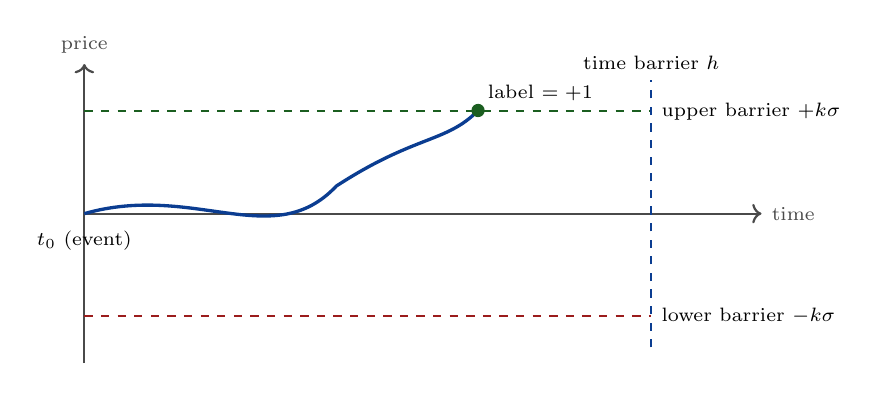
\begin{tikzpicture}[scale=1.0]
\draw[->,thick,msgrey] (0,0) -- (8.6,0) node[right,font=\scriptsize]{time};
\draw[->,thick,msgrey] (0,-1.9) -- (0,1.9) node[above,font=\scriptsize]{price};
\draw[dashed,msgreen,thick] (0,1.3) -- (7.2,1.3) node[right,font=\scriptsize,black]{upper barrier $+k\sigma$};
\draw[dashed,msred,thick]   (0,-1.3) -- (7.2,-1.3) node[right,font=\scriptsize,black]{lower barrier $-k\sigma$};
\draw[dashed,msblue,thick]  (7.2,-1.7) -- (7.2,1.7) node[above,font=\scriptsize,black]{time barrier $h$};
\draw[msblue,very thick] (0,0) .. controls (1.4,0.4) and (2.4,-0.5) .. (3.2,0.35)
                         .. controls (4.2,1.0) and (4.6,0.9) .. (5.0,1.31);
\fill[msgreen] (5.0,1.31) circle (2.4pt) node[above right,font=\scriptsize,black]{label $= +1$};
\node[font=\scriptsize,anchor=north] at (0,-0.1) {$t_0$ (event)};
\end{tikzpicture}
\end{center}

\begin{longtable}{@{}p{3.6cm}p{11.0cm}@{}}
\toprule
\textbf{Choice} & \textbf{Specification}\\
\midrule
Barriers & Upper and lower at $\pm k\sigma_t$ where $\sigma_t$ is the
\emph{current} volatility estimate (not a fixed point value). $k$ tuned per
horizon; start with $k=1.5$.\\
Time barrier & $h \in \{5, 15, 30\}$ minutes and always before the session close.\\
Label & $+1$ upper hit first, $-1$ lower hit first, $0$ time barrier hit.\\
Sample weights & Weight each sample by uniqueness (overlapping outcome windows
are not independent) and by absolute realised return.\\
Meta-labelling & A second model predicts \emph{whether the primary model's call
should be taken}. Primary model decides side; meta model decides size, including
size zero. This consistently improves precision.\\
\bottomrule
\end{longtable}

\begin{keybox}[title={Why triple-barrier changes the product}]
It directly encodes stop-loss and target into the label. A model trained this way
is answering the question you actually care about --- ``if I enter now with this
stop and this target, do I win?'' --- rather than an academic question about
candle colour.
\end{keybox}

\section{Cross-validation without lying to yourself}

\begin{longtable}{@{}p{3.8cm}p{10.8cm}@{}}
\toprule
\textbf{Technique} & \textbf{Why it is mandatory}\\
\midrule
Purged K-fold & Remove training samples whose outcome window overlaps the test
window. Without purging, the model sees the answer.\\
Embargo & Additionally drop a buffer (e.g. 1 trading day) after each test fold
to kill serial-correlation leakage.\\
Walk-forward (anchored and rolling) & The only evaluation that resembles
production. Report both.\\
Combinatorial purged CV & Generates many backtest paths, giving a
\emph{distribution} of Sharpe ratios rather than one lucky number.\\
Deflated Sharpe ratio & Corrects for the number of strategy variants tried.
If you tested 200 configurations, your best Sharpe is inflated --- quantify it.\\
Event-level splitting & Never split the same event's samples across train and
test. Group by event ID.\\
\bottomrule
\end{longtable}

\begin{warnbox}[title={Leakage checklist --- run before believing any result}]
\begin{enumerate}
\item Does any feature use data with a timestamp after the decision time?
\item Is normalisation (mean/std, scaler) fitted on the full dataset instead of
train only?
\item Are volatility estimates computed with a centred window?
\item Are labels from overlapping windows present in both train and test?
\item Was feature selection done before the split?
\item Does the news timestamp reflect publication or the time you downloaded it?
\item Is the option chain snapshot the one available at decision time, or the
end-of-day file?
\item Are corporate actions and index reconstitutions handled point-in-time?
\end{enumerate}
Any single ``yes'' invalidates the result. Most spectacular backtests die here.
\end{warnbox}

\section{Model portfolio}

Do not build one model. Build a small ensemble of models with genuinely
different inductive biases, then combine them.

\begin{longtable}{@{}p{3.2cm}p{3.4cm}p{7.8cm}@{}}
\toprule
\textbf{Model} & \textbf{Predicts} & \textbf{Role and notes}\\
\midrule
M0 Rules baseline & direction & Simple event-prior lookup plus momentum filter.
\textbf{Every ML model must beat this or it does not ship.} Also the
degraded-mode fallback.\\
M1 LightGBM & $P(\text{up})$, triple-barrier class & The workhorse. Handles
tabular heterogeneous features and missing values, trains in minutes, is
interpretable via SHAP. Expect this to be your best model for a long time.\\
M2 Quantile LightGBM & $q_{05},q_{25},q_{50},q_{75},q_{95}$ of $r_h$ &
Pinball loss. Feeds the fan chart directly.\\
M3 Temporal CNN / TCN & direction and magnitude & Learns local shape patterns
from raw candle and microstructure sequences that hand-crafted features miss.\\
M4 Sequence transformer & multi-horizon distribution & Attention over the last
$N$ minutes plus event tokens. Highest ceiling, highest overfitting risk, needs
the most data. \textbf{Build this last, not first.}\\
M5 Volatility model & $\sigma_{t+h}$ & HAR-RV baseline plus a gradient-boosting
correction on the residual. Volatility is the most forecastable target ---
give it a dedicated, well-tuned model.\\
M6 IV-change model & $\Delta\sigma_{IV}$ & Predicts implied volatility movement.
\textbf{Directly determines options profitability.} Features: current IV rank,
event class, term-structure slope, time to expiry, realised-implied spread.\\
M7 Meta-labeller & take / skip & Trained on primary model outputs plus market
state. Its job is to say no.\\
M8 Regime classifier & regime label & Hidden Markov model or clustering over
volatility, trend and liquidity. Everything else is conditioned on it.\\
\bottomrule
\end{longtable}

\section{Ensembling and calibration}

\begin{enumerate}
\item \term{Stacking with time-aware folds.} Out-of-fold predictions from
M1--M4 become inputs to a simple logistic regression meta-learner. Keep the
meta-learner simple; a complex stacker overfits immediately.
\item \term{Regime-conditional weights.} Model weights vary by regime from M8;
a transformer that shines in trending regimes may be useless in chop.
\item \term{Probability calibration.} Fit isotonic regression or Platt scaling on
a held-out, chronologically later slice. Then verify with a reliability diagram
and the Brier score decomposition (reliability, resolution, uncertainty).
\item \term{Conformal prediction.} Wrap the magnitude forecast in split conformal
intervals to obtain finite-sample coverage guarantees. When the interval is too
wide to be tradeable, the honest answer is no trade --- and now the system can
prove it.
\end{enumerate}

\begin{keybox}[title={The calibration contract}]
The dashboard's headline metric is not accuracy. It is the reliability diagram:
of all the times the system said 60\%, how often was it right? A system that is
calibrated can be sized correctly. A system that is accurate but overconfident
will still blow up.
\end{keybox}

\section{Training loop and retraining policy}

\begin{longtable}{@{}p{3.6cm}p{3.2cm}p{7.6cm}@{}}
\toprule
\textbf{Job} & \textbf{Cadence} & \textbf{Detail}\\
\midrule
Nightly feature materialisation & Daily 18:00 & Recompute the day's features,
run quality gates, append to Parquet.\\
Incremental retrain & Weekly (weekend) & Refit M1, M2, M5, M6 on the expanded
window; run walk-forward; promote only if it beats the incumbent on the
last 4 weeks out-of-sample.\\
Full retrain and architecture search & Quarterly & Includes M3/M4
hyperparameters and feature re-selection.\\
Impact library rebuild & Weekly & New events added; posteriors updated.\\
Calibration refresh & Weekly & Isotonic refit on the most recent 4 weeks.\\
Drift monitor & Continuous & PSI on features, KL divergence on prediction
distribution, rolling Brier score. Breach triggers alert and blocks
auto-execution.\\
Champion/challenger & Continuous & The challenger runs in shadow mode on live
data for at least 15 sessions before it may be promoted.\\
\bottomrule
\end{longtable}

\begin{warnbox}[title={Anti-overfitting discipline}]
Keep a \textbf{locked holdout}: the most recent 3 months of data, encrypted and
untouched. You may evaluate against it \emph{once}, at the Phase~7 gate.
Every additional peek burns the only honest estimate you will ever have.
Log every experiment; deflate your Sharpe by the number of trials.
\end{warnbox}

% =====================================================================
\chapter{Candle Projection: Honest Ghost Candles}
\label{ch:candles}
% =====================================================================

\section{The redesign}

The original design draws a single predicted OHLC sequence. That is
scientifically indefensible and, worse, psychologically dangerous: a crisp
predicted candle invites the user to bet as if it were certain.

The redesign keeps the visual drama and adds truth: draw a \term{probability
cone} made of quantile candles, where the body and wick widths encode
uncertainty and the colour intensity encodes directional confidence.

\begin{center}
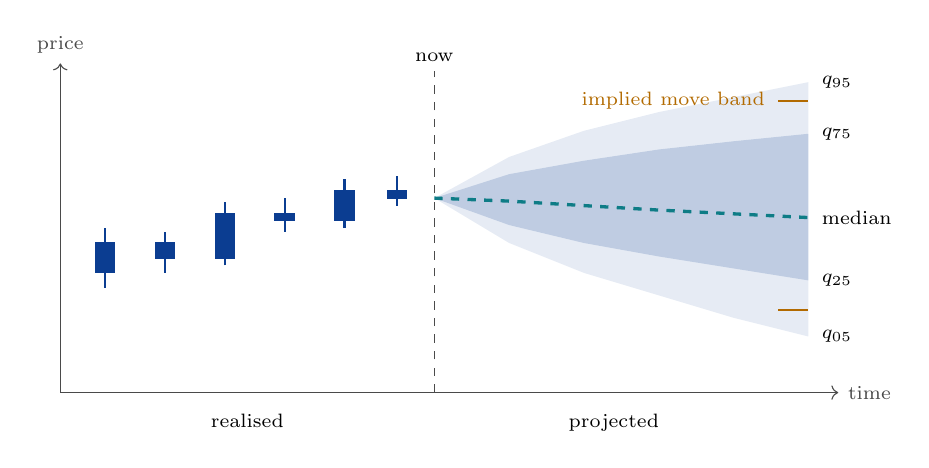
\begin{tikzpicture}[scale=0.95]
\draw[msgrey,->] (0,0) -- (10.4,0) node[right,font=\scriptsize]{time};
\draw[msgrey,->] (0,0) -- (0,4.4) node[above,font=\scriptsize]{price};
\node[font=\scriptsize,anchor=north] at (2.5,-0.15) {realised};
\node[font=\scriptsize,anchor=north] at (7.4,-0.15) {projected};
\draw[dashed,msgrey] (5.0,0) -- (5.0,4.3) node[above,font=\scriptsize,black]{now};

% realised candles
\foreach \x/\o/\c/\h/\l in {0.6/1.6/2.0/2.2/1.4, 1.4/2.0/1.8/2.15/1.6,
  2.2/1.8/2.4/2.55/1.7, 3.0/2.4/2.3/2.6/2.15, 3.8/2.3/2.7/2.85/2.2,
  4.5/2.7/2.6/2.9/2.5}{
  \draw[msblue,thick] (\x,\l) -- (\x,\h);
  \draw[msblue,fill=msblue] (\x-0.13,\o) rectangle (\x+0.13,\c);
}
% cone bands
\fill[msblue,opacity=0.10] (5.0,2.6) -- (6.0,3.15) -- (7.0,3.5) -- (8.0,3.75) -- (9.0,3.95) -- (10.0,4.15)
  -- (10.0,0.75) -- (9.0,1.0) -- (8.0,1.3) -- (7.0,1.6) -- (6.0,2.0) -- cycle;
\fill[msblue,opacity=0.18] (5.0,2.6) -- (6.0,2.92) -- (7.0,3.1) -- (8.0,3.25) -- (9.0,3.36) -- (10.0,3.46)
  -- (10.0,1.5) -- (9.0,1.66) -- (8.0,1.82) -- (7.0,2.0) -- (6.0,2.24) -- cycle;
\draw[mscyan,very thick,dashed] (5.0,2.6) -- (6.0,2.56) -- (7.0,2.50) -- (8.0,2.44) -- (9.0,2.39) -- (10.0,2.34);
\node[font=\scriptsize,anchor=west] at (10.05,4.15) {$q_{95}$};
\node[font=\scriptsize,anchor=west] at (10.05,3.46) {$q_{75}$};
\node[font=\scriptsize,anchor=west] at (10.05,2.34) {median};
\node[font=\scriptsize,anchor=west] at (10.05,1.50) {$q_{25}$};
\node[font=\scriptsize,anchor=west] at (10.05,0.75) {$q_{05}$};
% implied move markers
\draw[msamber,thick] (9.6,3.9) -- (10.0,3.9);
\draw[msamber,thick] (9.6,1.1) -- (10.0,1.1);
\node[font=\scriptsize,msamber,anchor=east] at (9.55,3.9) {implied move band};
\end{tikzpicture}
\end{center}

\section{How the cone is produced}

\begin{enumerate}
\item \term{Volatility forecast} $\hat\sigma_h$ from M5 (HAR-RV plus boosted
residual), conditioned on the event.
\item \term{Drift forecast} $\hat\mu_h$ from the calibrated direction ensemble
converted to an expected return: $\hat\mu_h = (2p_{\text{up}}-1)\cdot
\mathbb{E}[|r_h|]$, damped by the meta-labeller's confidence.
\item \term{Direct quantile heads} from M2 give $q_\alpha(r_h)$ for
$\alpha \in \{0.05,0.25,0.5,0.75,0.95\}$ at each horizon.
\item \term{Path sampling} for the visual: draw $N=5000$ paths from a
volatility-clustering process (a student-$t$ innovation GARCH-style simulator, or
a conditional generative model trained on real intraday paths) calibrated so the
terminal distribution matches the quantile heads. Then compute the per-minute
empirical quantiles of open, high, low and close.
\item \term{Rendering}: each projected minute is drawn as a semi-transparent
candle whose body spans $[q_{25}, q_{75}]$ of the close and whose wick spans
$[q_{05}, q_{95}]$, tinted by $P(\text{up})$.
\item \term{Overlay the implied move} from the option chain on the same axis.
When the cone is narrower than the implied move band, options are expensive
relative to our forecast --- that is a sell-volatility setup, and it is
immediately visible.
\end{enumerate}

\begin{keybox}[title={The killer visual}]
Two bands on one chart: \emph{what we forecast} versus \emph{what the market has
priced}. The gap between them is the trade. No competing retail product shows
this, and it makes the product's thesis legible in one glance.
\end{keybox}

\section{Scoring the projection honestly}

\begin{longtable}{@{}p{4.0cm}p{4.6cm}p{5.8cm}@{}}
\toprule
\textbf{Metric} & \textbf{Definition} & \textbf{Target}\\
\midrule
Pinball loss & Quantile loss averaged over $\alpha$ & Must beat a random-walk
baseline with GARCH volatility by at least 8\% relative.\\
CRPS & Continuous ranked probability score & Lower than both random walk and the
implied-volatility-derived distribution.\\
PIT histogram & Probability integral transform of realised outcomes & Should be
uniform. Humps at the edges mean intervals are too narrow.\\
Empirical coverage & Fraction of outcomes inside $[q_{05},q_{95}]$ & Within
$90\% \pm 3\%$.\\
Interval width efficiency & Mean width given coverage & Narrower is better only
if coverage holds.\\
Directional deviation & $|\text{realised} - \text{median}|$ & Reported, but
never as the headline metric.\\
\bottomrule
\end{longtable}

\begin{warnbox}[title={Reject the temptation}]
Do not display a single crisp predicted candle even if users ask for it. Instead
display the median path as a thin dashed line inside the cone. The moment the
product implies certainty, its users will size themselves into ruin and blame
the product --- correctly.
\end{warnbox}

% =====================================================================
\chapter{Options Recommendation Engine}
\label{ch:options}
% =====================================================================

\section{From a price forecast to a trade}

A forecast distribution over the underlying is not a trade. The engine performs
five steps.

\begin{center}
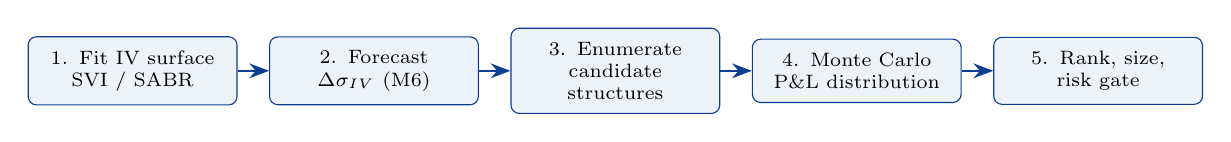
\begin{tikzpicture}[node distance=4mm and 4mm,blk/.append style={text width=2.3cm}]
\node[blk] (a) {1. Fit IV surface\\ SVI / SABR};
\node[blk,right=of a] (b) {2. Forecast\\ $\Delta\sigma_{IV}$ (M6)};
\node[blk,right=of b] (c) {3. Enumerate\\ candidate structures};
\node[blk,right=of c] (d) {4. Monte Carlo\\ P\&L distribution};
\node[blk,right=of d] (e) {5. Rank, size,\\ risk gate};
\draw[ar](a)--(b);\draw[ar](b)--(c);\draw[ar](c)--(d);\draw[ar](d)--(e);
\end{tikzpicture}
\end{center}

\section{Step 1 --- The implied volatility surface}

Raw per-strike implied volatilities from a live chain are noisy and occasionally
arbitrageable due to stale quotes. Fit a smooth, arbitrage-free surface:

\begin{itemize}
\item Compute implied volatility from mid prices only (never last traded price
--- a stale last price generates a fake signal), using Black-76 on futures or
Black--Scholes on spot with the appropriate forward.
\item Filter: bid $>0$, spread below a threshold, open interest above a
threshold, and $|\delta| \in [0.05, 0.95]$.
\item Fit a parametric slice per expiry (SVI is the standard choice), enforcing
no calendar and no butterfly arbitrage.
\item Store surface parameters, not just points. Slope, curvature and level
become features; the fitted surface prices any strike, including illiquid ones.
\end{itemize}

\section{Step 2 --- Forecasting the volatility change}

\begin{keybox}[title={The most valuable model in the system}]
$\Delta\sigma_{IV}$ over the next 15--30 minutes is more forecastable than
direction and it dominates short-dated option P\&L. Typical patterns to learn:
\begin{itemize}
\item Implied volatility \emph{expands} ahead of a scheduled event and
\emph{collapses} within minutes of the release --- regardless of direction.
\item After an unscheduled shock, implied volatility overshoots and mean-reverts
with a half-life measured in tens of minutes.
\item On expiry day, implied volatility decays mechanically and violently.
\item Elevated implied volatility rank means buying premium has a strong
headwind.
\end{itemize}
\end{keybox}

\section{Step 3 --- Candidate structures}

\begin{longtable}{@{}p{3.2cm}p{3.6cm}p{3.4cm}p{3.8cm}@{}}
\toprule
\textbf{Structure} & \textbf{Use when} & \textbf{Main risk} & \textbf{Notes}\\
\midrule
Long ATM/OTM call or put & Strong direction, forecast move well above implied,
implied volatility rank low & Vega and theta & Simple, highest gamma, but the
most exposed to volatility crush.\\
Vertical debit spread & Direction good, implied volatility elevated & Capped
upside & \textbf{Default directional structure post-news.} The short leg
neutralises much of the vega.\\
Long straddle / strangle & Big move expected, direction unclear, before a
scheduled event & Volatility crush if the move disappoints & Only when forecast
move exceeds implied move by a wide margin.\\
Short strangle with wings (iron condor) & Forecast move well below implied, calm
regime & Tail risk & Defined risk only. Never naked short options.\\
Calendar spread & Term structure dislocated & Complex & Advanced; phase 3 of the
options engine.\\
Ratio / broken-wing & Skew dislocation & Asymmetric & Advanced.\\
\textbf{No trade} & Forecast within noise of implied & --- & Must be the most
frequently selected option.\\
\bottomrule
\end{longtable}

Strike selection is constrained, not free: only strikes with adequate open
interest, adequate volume in the last five minutes, and a bid-ask spread below a
fraction of the option price are eligible. A theoretically optimal strike that
cannot be exited is a trap.

\section{Step 4 --- Monte Carlo P\&L distribution}

For each candidate structure:

\begin{enumerate}
\item Take the $N$ sampled underlying paths from Chapter~\ref{ch:candles}.
\item For each path and each future minute, evolve the implied volatility surface
using the M6 forecast plus a stochastic component (correlated negatively with
the underlying for equity indices --- the leverage effect).
\item Reprice the structure along the path, including the passage of time.
\item Apply the exit rule (target, stop, time stop) to get a realised P\&L per
path.
\item Subtract full transaction costs on both legs, entry and exit, including
modelled slippage as a function of the spread and size.
\end{enumerate}

The output is a P\&L distribution, from which we extract:

\[
\mathbb{E}[\text{P\&L}],\quad
P(\text{profit}),\quad
\text{CVaR}_{5\%},\quad
\frac{\mathbb{E}[\text{P\&L}]}{\text{std}},\quad
\text{max drawdown along the path}.
\]

\begin{keybox}[title={Ranking objective}]
Rank by risk-adjusted expected value after costs, penalised by illiquidity:
\[
\text{Score} = \frac{\mathbb{E}[\text{P\&L}] - \lambda\,\text{CVaR}_{5\%}}
{\text{capital at risk}} \cdot \underbrace{\Big(1 - \tfrac{\text{spread}}{2\,\text{mid}}\Big)^2}_{\text{liquidity penalty}}
\]
Emit a recommendation only if $\mathbb{E}[\text{P\&L}] > 0$ after costs
\emph{and} the score exceeds a minimum threshold \emph{and} the meta-labeller
approves.
\end{keybox}

\section{Step 5 --- Position sizing}

Never size by intuition or by a fixed lot count. Use fractional Kelly with a hard
cap:

\[
f^{*} = \frac{p\,b - (1-p)}{b}, \qquad
f_{\text{used}} = \min\!\Big(0.25\,f^{*},\; f_{\max}\Big)
\]

where $p$ is the calibrated win probability, $b$ the payoff ratio from the Monte
Carlo, $0.25$ is the fractional-Kelly discount (full Kelly is far too aggressive
when $p$ is estimated), and $f_{\max}$ is a hard per-trade cap (start at 1--2\%
of capital risked).

\begin{longtable}{@{}p{4.8cm}p{9.8cm}@{}}
\toprule
\textbf{Additional size modifier} & \textbf{Effect}\\
\midrule
Posterior uncertainty of the impact prior & Size scales with
$1/\sqrt{1 + \text{var}}$; small sample sizes shrink the position.\\
Regime & Reduce size in high-volatility or low-liquidity regimes.\\
Time of day & Reduce size in the first 10 and last 15 minutes.\\
Consecutive losses & Reduce size after a losing streak (anti-martingale).\\
Correlation with open positions & Aggregate delta and vega across the book, not
per trade.\\
Expiry day & Halve size; gamma risk is extreme.\\
\bottomrule
\end{longtable}

\section{Complete recommendation record}

Every recommendation is an immutable, fully-explained record. This is both the
product's differentiator and the audit trail.

\begin{lstlisting}[language=Python,caption={Recommendation schema}]
{
  "reco_id": "uuid", "trace_id": "uuid",         # links back to the news item
  "ts_emitted": "2026-08-26T09:20:41.318+05:30",
  "trigger": {"event_id": "...", "class": "geopolitical.military_action",
              "severity_cal": 8.2, "novelty": 0.91, "credibility": 0.88,
              "sources": ["src_a","src_b"], "seconds_since_event": 4.1},
  "forecast": {"horizon_min": 15,
               "p_up": 0.31, "p_up_ci": [0.24, 0.39],
               "quantiles": {"q05": -0.0142, "q25": -0.0071, "q50": -0.0033,
                             "q75": 0.0004, "q95": 0.0061},
               "sigma_forecast": 0.0089, "d_iv_forecast": +2.4,
               "implied_move_15m": 0.0052, "edge_ratio": 1.71},
  "structure": {"type": "bear_put_debit_spread",
                "legs": [{"side":"BUY","strike":19500,"opt":"PE","qty":1},
                         {"side":"SELL","strike":19300,"opt":"PE","qty":1}],
                "net_debit": 78.5, "max_profit": 121.5, "max_loss": 78.5,
                "breakeven": 19421.5},
  "greeks_net": {"delta": -0.21, "gamma": 0.0009, "vega": -1.8, "theta": -3.1},
  "mc": {"paths": 5000, "E_pnl": 21.4, "p_profit": 0.57,
         "cvar5": -71.2, "score": 0.184},
  "sizing": {"kelly_frac": 0.061, "used_frac": 0.015, "lots": 2,
             "capital_at_risk": 11775},
  "exits": {"target": 121.5, "stop": -39.0, "time_stop": "09:36:00",
            "vol_stop": "exit if IV drops > 3 pts"},
  "explanation": ["Military escalation, severity 8.2, first mention 4.1s ago",
                  "Historical prior for this class: median -0.31% over 15m (n=23)",
                  "Forecast |move| 1.71x implied move -> premium buying justified",
                  "IV rank 62 -> spread chosen over naked put to cut vega",
                  "Dealer gamma negative -> moves amplify"],
  "gates_passed": ["credibility>=0.8","two_sources","not_already_priced",
                   "liquidity_ok","daily_loss_limit_ok","regime_ok"],
  "model_versions": {"cls":"ev-cls-v7","dir":"ens-v12","vol":"har-gb-v4",
                     "iv":"ivd-v3","meta":"meta-v5"},
  "mode": "PAPER"
}
\end{lstlisting}

\begin{keybox}[title={Why the explanation field is not decoration}]
Six months from now you will be trying to find out why the system lost money on
a class of events. Without a stored, structured reason for every decision, that
investigation is impossible and the system cannot improve. The explanation array
is a first-class engineering requirement, not a UI nicety.
\end{keybox}

% =====================================================================
\chapter{Risk Management and Kill Switches}
\label{ch:risk}
% =====================================================================

\section{The risk gate sits between the brain and the money}

No component may bypass the risk gate. It is deliberately simple, deliberately
conservative, and deliberately hard to change (changes require a written
justification recorded in the repository).

\begin{longtable}{@{}p{4.4cm}p{3.0cm}p{7.0cm}@{}}
\toprule
\textbf{Limit} & \textbf{Starting value} & \textbf{Behaviour on breach}\\
\midrule
Per-trade capital at risk & 1.5\% & Reject or resize down.\\
Daily loss limit & 3\% & \textbf{Stop for the day.} Flatten everything. No
overrides.\\
Weekly loss limit & 6\% & Stop for the week; mandatory review before restart.\\
Max concurrent positions & 2 & Reject new signals.\\
Net portfolio delta & bounded band & Reject trades that increase concentration.\\
Net portfolio vega & bounded band & Prevents accidental all-in volatility bets.\\
Max trades per day & 6 & Prevents overtrading in a noisy news day.\\
Max trades per event & 1 & Prevents pyramiding on one hypothesis.\\
Slippage guard & 0.5\% of premium & Cancel if fill price deviates.\\
Time-of-day block & first 5 min, last 10 min & No new entries.\\
Expiry-day multiplier & 0.5x size & Gamma risk.\\
Model degraded flag & any & Signals become advisory only.\\
Data staleness & feed silent 3 s & Halt everything.\\
\bottomrule
\end{longtable}

\section{Kill switch hierarchy}

\begin{longtable}{@{}p{2.2cm}p{4.0cm}p{8.4cm}@{}}
\toprule
\textbf{Level} & \textbf{Trigger} & \textbf{Action}\\
\midrule
L1 Soft & Drift alert, calibration decay, unusual latency & Reduce size by half;
notify.\\
L2 Pause & Daily loss limit, data quality failure, conflicting events &
Stop new entries; manage existing positions only.\\
L3 Flatten & Feed loss, model server failure, clock drift, retraction of the
triggering news & Close all positions at market immediately; stop.\\
L4 Lockout & Two L3 events in a week, or any unexplained loss & System refuses to
run until a human clears it with a written root-cause note.\\
\bottomrule
\end{longtable}

\begin{warnbox}[title={Physical kill switch}]
Provide a single command and a single dashboard button that flattens everything
and disables the system, requiring no dependency on the very components that may
have failed. Test it monthly. Also test what happens when the broker API returns
an error during the flatten --- that is the scenario that actually costs money.
\end{warnbox}

\section{Scenario stress tests (run before each promotion)}

\begin{enumerate}
\item Circuit breaker: the index hits a limit and trading halts mid-position.
\item Flash crash and instant recovery within 90 seconds.
\item Broker API returns success but the order was not placed.
\item Duplicate order acknowledgement (double fill).
\item Option chain goes stale but the spot feed stays live.
\item A false catastrophic headline followed by a retraction 4 minutes later.
\item Two contradictory high-severity events 20 seconds apart.
\item Expiry-day final 30 minutes with implied volatility collapsing.
\item Internet loss for 45 seconds with an open position.
\item Model server returns predictions from a stale model version.
\end{enumerate}

For each: define the expected behaviour, implement it, and write an automated
replay test. A system that has not been tested against these has not been
tested.

% =====================================================================
\chapter{Backtesting and Simulation}
\label{ch:backtest}
% =====================================================================

\section{Three levels of simulation}

\begin{longtable}{@{}p{2.6cm}p{4.2cm}p{7.8cm}@{}}
\toprule
\textbf{Level} & \textbf{What it is} & \textbf{What it can and cannot tell you}\\
\midrule
L1 Vectorised & Fast pandas/DuckDB evaluation over historical features and
labels & Fast model iteration and feature screening. \textbf{Cannot} model
execution, latency or queue position. Never trust a P\&L number from here.\\
L2 Event-driven & A simulator that replays ticks, news and chain snapshots in
timestamp order through the actual production code path & The real answer.
Models latency, partial fills, spread, stale quotes, exits. Slow but honest.\\
L3 Live paper & The production system running on live data with simulated fills
& Catches everything L2 misses: real feed hiccups, real API errors, real
timing. \textbf{The only evidence that counts for the Phase~7 gate.}\\
\bottomrule
\end{longtable}

\begin{keybox}[title={Rule}]
Model research happens at L1. \emph{Every claim about profitability} must come
from L2, and \emph{every go-live decision} must come from L3. A number produced
at L1 may never appear in a slide about returns.
\end{keybox}

\section{The event-driven simulator}

\begin{lstlisting}[language=Python,caption={Simulator core loop (conceptual)}]
# Single merged, timestamp-ordered stream. This ordering IS the correctness
# guarantee: nothing can be consumed before its t_available.
for msg in merged_stream(ticks, chain_snaps, news, calendar, start, end):
    clock.set(msg.ts)
    bus.publish(msg)                      # same bus code as production
    for out in engine.drain():            # same engine code as production
        if out.kind == "reco":
            broker_sim.submit(out, latency=sample_latency(),
                              slippage=slippage_model(out, book_state))
    broker_sim.mark_to_market(clock.now())
    risk.check(clock.now())
\end{lstlisting}

\begin{longtable}{@{}p{4.0cm}p{10.6cm}@{}}
\toprule
\textbf{Realism requirement} & \textbf{Implementation}\\
\midrule
Decision latency & Inject a sampled delay between event timestamp and the
moment the engine is allowed to act. Draw from the measured live latency
distribution, not a constant.\\
Fill model & Marketable orders fill at the far touch plus a slippage term that
grows with size relative to displayed depth and with spread width. Limit orders
fill only if the market trades through them, with a queue-position discount.\\
Partial fills & Multi-lot orders may partially fill; the engine must handle it.\\
Stale quotes & If the last chain snapshot is older than $x$ seconds, the
simulator refuses the trade, exactly as production must.\\
Costs & Full stack: brokerage, exchange transaction charge, STT/CTT, SEBI fee,
GST, stamp duty, plus modelled slippage. Rates change --- keep them in a dated
configuration table, applied point-in-time.\\
Impact & For retail size in index options, market impact is small but not zero;
model it as a function of order size relative to trailing volume.\\
Exits & Simulated with intrabar path assumptions that are \emph{conservative}:
if both target and stop are touched within the same minute, assume the stop
filled first.\\
\bottomrule
\end{longtable}

\begin{warnbox}[title={The conservative-tie rule}]
The stop-first assumption on ambiguous bars typically reduces backtest returns by
a large margin. Keep it. Every optimistic assumption you allow is a loan you
repay with real money later.
\end{warnbox}

\section{Cost model}

\begin{longtable}{@{}p{4.6cm}p{4.2cm}p{5.6cm}@{}}
\toprule
\textbf{Component} & \textbf{Applies to} & \textbf{Modelling note}\\
\midrule
Brokerage & Per executed order & Flat per order for most discount brokers; a
two-leg spread entered and exited is four orders.\\
Exchange transaction charge & Premium turnover & Percentage of premium.\\
Securities transaction tax & Sell side (and exercised options) & Materially
different on expiry if allowed to expire in the money --- \textbf{always square
off, never let ITM options expire.}\\
Regulator fee, stamp duty & Turnover & Small but included.\\
GST & On brokerage plus charges & Included.\\
Slippage & Every fill & The dominant real-world cost. Estimate from your own
live paper fills, not from theory.\\
\bottomrule
\end{longtable}

\begin{keybox}[title={The breakeven reality check}]
Compute your all-in round-trip cost as a percentage of the option premium at
entry. For small premiums and multi-leg structures this can be several percent.
The engine must require $\mathbb{E}[\text{P\&L}]$ to exceed this by a
comfortable margin --- otherwise the strategy is a machine for converting edge
into fees.
\end{keybox}

% =====================================================================
\chapter{Evaluation Framework}
\label{ch:eval}
% =====================================================================

\section{Metric hierarchy}

Metrics are organised by what decision they inform. Do not mix layers.

\begin{longtable}{@{}p{2.6cm}p{4.2cm}p{7.8cm}@{}}
\toprule
\textbf{Layer} & \textbf{Metrics} & \textbf{Decision it drives}\\
\midrule
Detection & Precision, recall, macro-F1 per event class; first-mention latency;
duplicate rate; false-positive rate on the noise class & Should the classifier
ship?\\
Impact & Coverage of predicted intervals; correlation of predicted and realised
abnormal return; sample sizes & Is the impact library trustworthy?\\
Forecast & Brier score and decomposition; reliability slope and intercept;
log loss; AUC; pinball loss; CRPS; PIT uniformity & Is the model calibrated?\\
Decision & Hit rate, payoff ratio, expectancy per trade, edge realisation
(realised versus predicted edge) & Is the decision layer converting forecasts
into good trades?\\
Portfolio & Net P\&L after costs, profit factor, Sharpe, Sortino, max drawdown,
Calmar, exposure time, turnover, cost drag & Should we scale capital?\\
Operational & p50/p99 latency per stage, uptime during market hours, data
completeness, error budget & Is the system healthy?\\
\bottomrule
\end{longtable}

\section{The attribution table --- the most useful report you will build}

Every trade is tagged with its event class, regime, time bucket, structure type,
horizon and model version. The weekly report then answers questions such as:

\begin{longtable}{@{}p{4.4cm}rrrrp{3.2cm}@{}}
\toprule
\textbf{Event class} & \textbf{$n$} & \textbf{Hit \%} & \textbf{Avg R} &
\textbf{Net} & \textbf{Verdict}\\
\midrule
monetary.rate\_decision & 12 & 66.7 & +0.81 & positive & Keep, size up\\
macro.inflation\_release & 19 & 57.9 & +0.34 & positive & Keep\\
geopolitical.rhetoric & 31 & 45.2 & $-0.22$ & negative & \textbf{Disable this
class}\\
energy.supply\-\_disruption & 7 & 57.1 & +0.11 & flat & Insufficient sample\\
flows.expiry\_pinning & 14 & 71.4 & +0.62 & positive & Keep, investigate scaling\\
\bottomrule
\end{longtable}

\begin{keybox}[title={Class-level kill policy}]
Any event class with at least 25 trades and negative expectancy over a rolling
quarter is \textbf{automatically disabled} by the system, not by a human debate.
Re-enabling requires a documented model change and a fresh out-of-sample
period. This single policy does more for long-run profitability than any model
improvement.
\end{keybox}

\section{The public accuracy dashboard, done properly}

The original dashboard shows ``32/47 correct (68\%)''. Replace with:

\begin{longtable}{@{}p{4.6cm}p{9.8cm}@{}}
\toprule
\textbf{Panel} & \textbf{Content}\\
\midrule
Reliability curve & Predicted probability bucket versus realised frequency, with
confidence bands and the count in each bucket.\\
Rolling Brier skill score & Versus a climatological baseline; the honest measure
of whether the model adds information.\\
Interval coverage & Realised coverage of the 50\% and 90\% bands over the
trailing 20 sessions.\\
Edge realisation & Scatter of predicted edge versus realised edge per trade;
the regression slope should be near 1. A slope near 0 means the model has no
usable edge regardless of hit rate.\\
Cost drag & Gross versus net P\&L, so cost erosion is always visible.\\
Drawdown curve & Underwater plot with the current position on the risk ladder.\\
Latency histogram & Per stage, p50/p95/p99, refreshed live.\\
Per-class attribution & The table above, always visible.\\
\bottomrule
\end{longtable}

% =====================================================================
\chapter{MLOps, Infrastructure and Operations}
\label{ch:mlops}
% =====================================================================

\section{Environments}

\begin{longtable}{@{}p{2.8cm}p{3.6cm}p{8.2cm}@{}}
\toprule
\textbf{Env} & \textbf{Data} & \textbf{Purpose}\\
\midrule
\texttt{research} & Historical Parquet & Notebooks, feature exploration, model
training. No connection to any broker credential, ever.\\
\texttt{replay} & Recorded live days & Deterministic regression testing of the
full pipeline. CI runs a fixed golden day on every commit.\\
\texttt{paper} & Live feeds & Production code, simulated fills. Runs every
session from Phase~5 onward.\\
\texttt{live} & Live feeds & Real orders. Separate credentials, separate
machine, separate alerting, stricter limits.\\
\bottomrule
\end{longtable}

\section{The daily operating rhythm}

\begin{longtable}{@{}p{2.4cm}p{4.0cm}p{8.2cm}@{}}
\toprule
\textbf{Time (IST)} & \textbf{Job} & \textbf{Detail}\\
\midrule
06:30 & Overnight digest & Collect global overnight events, compute the gap
forecast, publish the pre-market briefing.\\
08:45 & Preflight & Feed connectivity, clock sync, model version check, margin
check, calendar check (holiday, expiry, special session). Fails loudly.\\
09:00--09:15 & Pre-open watch & Observe only; no signals.\\
09:15--15:30 & Live session & Hot and cold lanes active; risk gate armed.\\
15:20 & Forced flatten & All intraday positions squared off; no exceptions.\\
15:45 & Post-session & Compute outcomes for every prediction, update the ledger,
run attribution, push metrics.\\
18:00 & Nightly & Feature materialisation, data-quality gates, archive to
Parquet, backup verification.\\
Weekend & Retrain & Incremental retrain, walk-forward, champion/challenger
evaluation, calibration refresh, weekly report generation.\\
\bottomrule
\end{longtable}

\section{Observability}

\begin{itemize}
\item \term{Trace ID propagation.} One identifier flows from the raw news item
through classification, features, prediction, recommendation and fill. Any
recommendation can be reconstructed end to end in one query. This is
non-negotiable for debugging a system with this many stages.
\item \term{Golden signals per plane:} latency, throughput, error rate,
saturation.
\item \term{Business alarms:} no signal emitted for two consecutive sessions
(system silently broken), signal rate three times the normal rate (classifier
gone haywire), calibration slope outside $[0.8, 1.2]$, feature null rate spike.
\item \term{Every prediction is logged with its feature vector hash} so that
post-hoc analysis can recompute exactly what the model saw.
\end{itemize}

\section{Reproducibility}

\begin{longtable}{@{}p{3.6cm}p{11.0cm}@{}}
\toprule
\textbf{Artifact} & \textbf{Discipline}\\
\midrule
Code & Git; every model artifact records the commit hash.\\
Data & Immutable, dated Parquet partitions; a dataset version is a manifest of
file hashes.\\
Features & Versioned definitions; changing a feature's logic requires a version
bump, never an in-place edit.\\
Models & MLflow registry with stage transitions (staging, shadow, production,
archived). Production reads only from the registry.\\
Config & All thresholds in versioned YAML, loaded at startup, hash logged.
No magic numbers in code.\\
Randomness & Seeded everywhere; the simulator is deterministic given a seed.\\
\bottomrule
\end{longtable}

\section{Security}

\begin{itemize}
\item Broker credentials and API keys in a secrets manager, never in the
repository, never in a notebook, never in an environment file committed by
accident. Add a pre-commit secret scanner on day one.
\item The live trading process runs on a separate host with a minimal
attack surface and no inbound ports except an authenticated control channel.
\item Two-person rule (or a written checklist plus a delay) for changing risk
limits.
\item All order-placing code paths require an explicit \texttt{live=True}
argument that defaults to \texttt{False} in every environment.
\item Immutable audit log of every order intent, shipped off-host.
\end{itemize}

% =====================================================================
\chapter{Dashboard and Product Surface}
\label{ch:ui}
% =====================================================================

\section{Design brief}

The dashboard has one job: let a human decide in three seconds whether to act,
and let the same human audit six weeks later why the machine acted. Everything
else is decoration.

\begin{center}
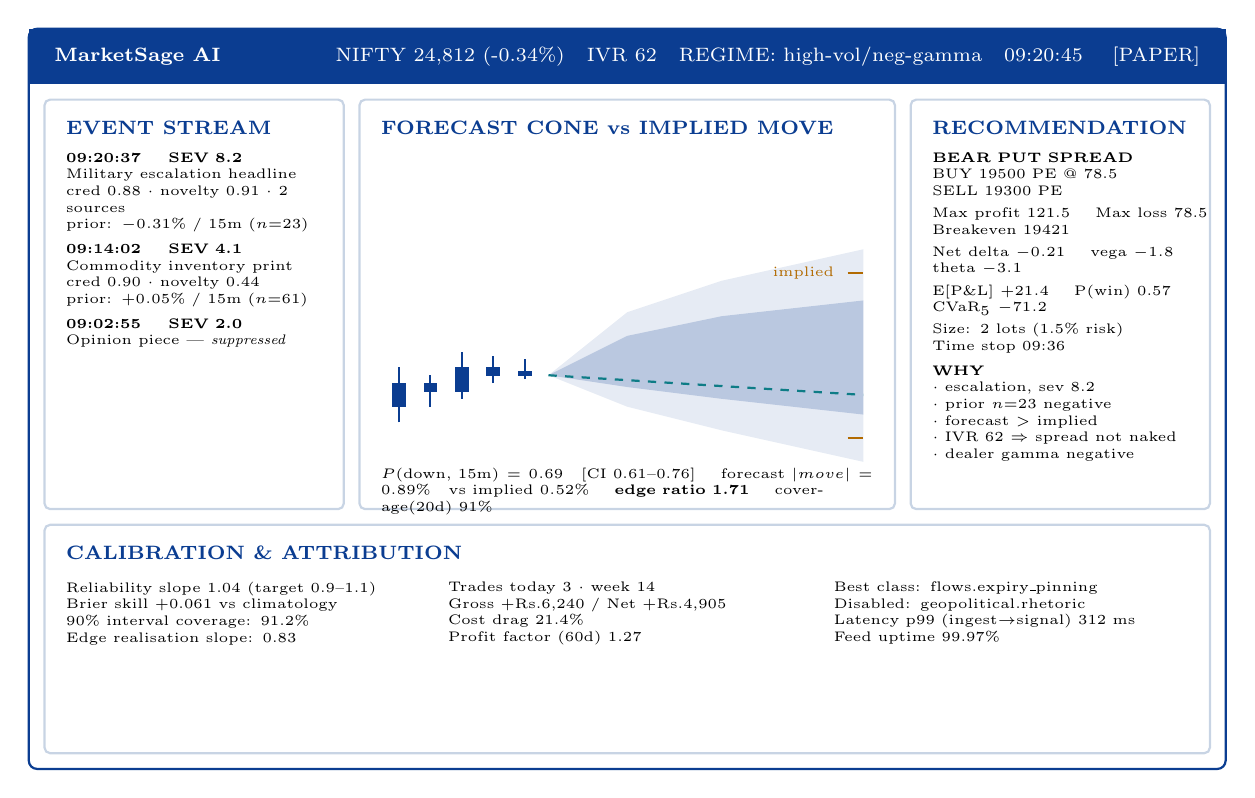
\begin{tikzpicture}[scale=1.0]
\draw[msblue,thick,rounded corners=3pt] (0,0) rectangle (15.2,9.4);
\fill[msblue] (0,8.7) rectangle (15.2,9.4);
\node[white,font=\scriptsize\bfseries,anchor=west] at (0.2,9.05)
  {MarketSage AI};
\node[white,font=\scriptsize,anchor=east] at (15.0,9.05)
  {NIFTY 24{,}812 (-0.34\%)\quad IVR 62\quad REGIME: high-vol/neg-gamma\quad 09:20:45 \quad [PAPER]};

% left column
\draw[msline,thick,rounded corners=2pt] (0.2,3.3) rectangle (4.0,8.5);
\node[font=\scriptsize\bfseries,msblue,anchor=north west] at (0.35,8.35) {EVENT STREAM};
\node[font=\tiny,anchor=north west,text width=3.5cm] at (0.35,7.95)
 {\textbf{09:20:37 \quad SEV 8.2}\\ Military escalation headline\\
  cred 0.88 $\cdot$ novelty 0.91 $\cdot$ 2 sources\\
  prior: $-0.31\%$ / 15m ($n{=}23$)\\[3pt]
  \textbf{09:14:02 \quad SEV 4.1}\\ Commodity inventory print\\
  cred 0.90 $\cdot$ novelty 0.44\\
  prior: $+0.05\%$ / 15m ($n{=}61$)\\[3pt]
  \textbf{09:02:55 \quad SEV 2.0}\\ Opinion piece --- \emph{suppressed}};

% centre
\draw[msline,thick,rounded corners=2pt] (4.2,3.3) rectangle (11.0,8.5);
\node[font=\scriptsize\bfseries,msblue,anchor=north west] at (4.35,8.35)
 {FORECAST CONE vs IMPLIED MOVE};
\fill[msblue,opacity=0.10] (6.6,5.0) -- (7.6,5.8) -- (8.8,6.2) -- (10.6,6.6)
   -- (10.6,3.9) -- (8.8,4.3) -- (7.6,4.6) -- cycle;
\fill[msblue,opacity=0.20] (6.6,5.0) -- (7.6,5.5) -- (8.8,5.75) -- (10.6,5.95)
   -- (10.6,4.5) -- (8.8,4.7) -- (7.6,4.85) -- cycle;
\draw[mscyan,thick,dashed] (6.6,5.0) -- (10.6,4.75);
\draw[msamber,thick] (10.4,6.3) -- (10.6,6.3);
\draw[msamber,thick] (10.4,4.2) -- (10.6,4.2);
\node[font=\tiny,msamber,anchor=east] at (10.35,6.3) {implied};
\foreach \x/\o/\c/\h/\l in {4.7/4.6/4.9/5.1/4.4, 5.1/4.9/4.8/5.0/4.6,
  5.5/4.8/5.1/5.3/4.7, 5.9/5.1/5.0/5.25/4.9, 6.3/5.0/5.05/5.2/4.95}{
  \draw[msblue,thick] (\x,\l)--(\x,\h);
  \draw[msblue,fill=msblue] (\x-0.08,\o) rectangle (\x+0.08,\c);}
\node[font=\tiny,anchor=north west,text width=6.4cm] at (4.35,3.95)
 {$P(\text{down, 15m}) = 0.69$ \; [CI 0.61--0.76] \quad
  forecast $|move| = 0.89\%$ \; vs implied $0.52\%$ \quad
  \textbf{edge ratio 1.71} \quad coverage(20d) 91\%};

% right
\draw[msline,thick,rounded corners=2pt] (11.2,3.3) rectangle (15.0,8.5);
\node[font=\scriptsize\bfseries,msblue,anchor=north west] at (11.35,8.35) {RECOMMENDATION};
\node[font=\tiny,anchor=north west,text width=3.5cm] at (11.35,7.95)
 {\textbf{BEAR PUT SPREAD}\\ BUY 19500 PE @ 78.5\\ SELL 19300 PE\\[2pt]
  Max profit 121.5 \quad Max loss 78.5\\ Breakeven 19421\\[2pt]
  Net delta $-0.21$ \quad vega $-1.8$\\ theta $-3.1$\\[2pt]
  E[P\&L] $+21.4$ \quad P(win) 0.57\\ CVaR$_{5}$ $-71.2$\\[2pt]
  Size: 2 lots (1.5\% risk)\\ Time stop 09:36\\[3pt]
  \textbf{WHY}\\ $\cdot$ escalation, sev 8.2\\ $\cdot$ prior $n{=}23$ negative\\
  $\cdot$ forecast $>$ implied\\ $\cdot$ IVR 62 $\Rightarrow$ spread not naked\\
  $\cdot$ dealer gamma negative};

% bottom
\draw[msline,thick,rounded corners=2pt] (0.2,0.2) rectangle (15.0,3.1);
\node[font=\scriptsize\bfseries,msblue,anchor=north west] at (0.35,2.95) {CALIBRATION \& ATTRIBUTION};
\node[font=\tiny,anchor=north west,text width=4.6cm] at (0.35,2.5)
 {Reliability slope 1.04 (target 0.9--1.1)\\ Brier skill +0.061 vs climatology\\
  90\% interval coverage: 91.2\%\\ Edge realisation slope: 0.83};
\node[font=\tiny,anchor=north west,text width=4.6cm] at (5.2,2.5)
 {Trades today 3 $\cdot$ week 14\\ Gross +\rs 6{,}240 / Net +\rs 4{,}905\\
  Cost drag 21.4\%\\ Profit factor (60d) 1.27};
\node[font=\tiny,anchor=north west,text width=4.6cm] at (10.1,2.5)
 {Best class: flows.expiry\_pinning\\ Disabled: geopolitical.rhetoric\\
  Latency p99 (ingest$\to$signal) 312 ms\\ Feed uptime 99.97\%};
\end{tikzpicture}
\end{center}

\section{Panels and their non-negotiable elements}

\begin{longtable}{@{}p{3.4cm}p{11.2cm}@{}}
\toprule
\textbf{Panel} & \textbf{Must contain}\\
\midrule
Event stream & Severity, credibility, novelty, source count, the historical prior
\emph{with its sample size}, and suppressed events shown greyed out so the user
sees what the system chose to ignore.\\
Forecast cone & The quantile bands, the median as a thin dashed line, the
implied-move band for comparison, the edge ratio, and the trailing coverage
statistic so the user knows whether to trust the bands today.\\
Recommendation & The full structure with both legs, net Greeks, the Monte Carlo
summary, the sizing rationale, all three exits (target, stop, time), and the
ordered ``why'' list.\\
Calibration \& attribution & Always visible, never hidden behind a tab. The
system's honesty is the product.\\
Status bar & Mode (PAPER/LIVE/DEGRADED), regime, latency, feed health. Mode must
be impossible to misread --- a full-width coloured band when live.\\
\bottomrule
\end{longtable}

\begin{keybox}[title={Interaction rules}]
\begin{itemize}
\item Nothing flashes or animates except a genuinely new high-severity event.
\item Every number is hoverable to reveal its computation and its as-of
timestamp.
\item Any recommendation can be opened into a full replay: the news item, the
feature vector, the model versions, the Monte Carlo distribution.
\item A permanent, unmissable indicator of PAPER versus LIVE mode.
\end{itemize}
\end{keybox}

\section{Alerting}

\begin{longtable}{@{}p{3.2cm}p{3.4cm}p{7.8cm}@{}}
\toprule
\textbf{Alert} & \textbf{Channel} & \textbf{Rule}\\
\midrule
Tradeable signal & Push + sound & Only when all gates pass. Rate-limited to
avoid alert fatigue.\\
High-severity event, no trade & Push, silent & ``Something is happening, risk is
elevated'' --- valuable even without a trade.\\
Position exit & Push & Target, stop or time stop hit.\\
Risk breach & Push + SMS & Any L2/L3 kill switch.\\
System health & Email/chat & Daily digest; immediate only for L3.\\
Calibration decay & Daily digest & Slow-moving; does not need to interrupt.\\
\bottomrule
\end{longtable}

% =====================================================================
\chapter{Phase-Gated Execution Roadmap}
\label{ch:roadmap}
% =====================================================================

\section{How to read this chapter}

Ten phases. Each has an objective, workstreams, checkpoints, a numeric
\term{exit gate}, and \term{kill criteria}. You may not begin phase $n+1$ until
phase $n$'s gate is signed off in writing (a dated entry in
\texttt{docs/gates.md} with the measured numbers pasted in).

The durations assume one committed developer working roughly 25--30 focused
hours per week. With a second person on data engineering, compress by around
30\%. Do not compress by skipping gates.

\begin{center}
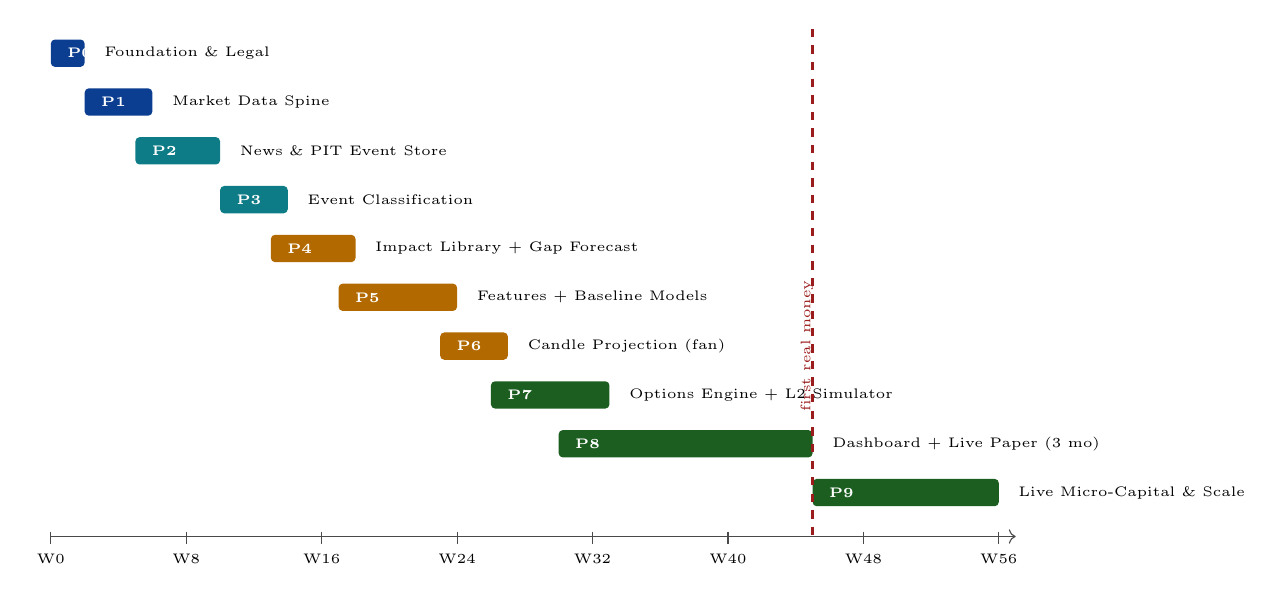
\begin{tikzpicture}[xscale=0.215,yscale=0.62]
\definecolor{barA}{HTML}{0B3D91}\definecolor{barB}{HTML}{0E7C86}
\definecolor{barC}{HTML}{B26A00}\definecolor{barD}{HTML}{1B5E20}
\foreach \p/\s/\e/\y/\col/\lab in {
  P0/0/2/0/barA/{Foundation \& Legal},
  P1/2/6/-1/barA/{Market Data Spine},
  P2/5/10/-2/barB/{News \& PIT Event Store},
  P3/10/14/-3/barB/{Event Classification},
  P4/13/18/-4/barC/{Impact Library + Gap Forecast},
  P5/17/24/-5/barC/{Features + Baseline Models},
  P6/23/27/-6/barC/{Candle Projection (fan)},
  P7/26/33/-7/barD/{Options Engine + L2 Simulator},
  P8/30/45/-8/barD/{Dashboard + Live Paper (3 mo)},
  P9/45/56/-9/barD/{Live Micro-Capital \& Scale}}{
  \fill[\col,rounded corners=1.5pt] (\s,\y-0.28) rectangle (\e,\y+0.28);
  \node[font=\tiny\bfseries,white,anchor=west] at (\s+0.4,\y) {\p};
  \node[font=\tiny,anchor=west,black] at (\e+0.6,\y) {\lab};
}
\draw[msgrey,->] (0,-9.9) -- (57,-9.9);
\foreach \w in {0,8,16,24,32,40,48,56}{
  \draw[msgrey] (\w,-9.8)--(\w,-10.05);
  \node[font=\tiny,anchor=north] at (\w,-10.05) {W\w};}
\draw[msred,dashed,thick] (45,0.5) -- (45,-9.9);
\node[font=\tiny,msred,anchor=south,rotate=90] at (45.6,-6) {first real money};
\end{tikzpicture}
\end{center}

% ---------------------------------------------------------------------
\section{Phase 0 --- Foundation and Legal (Weeks 1--2)}

\textbf{Objective.} Make it impossible to build the wrong thing, and start the
data clock.

\begin{longtable}{@{}p{1.4cm}p{6.0cm}p{7.0cm}@{}}
\toprule
\textbf{CP} & \textbf{Checkpoint} & \textbf{Definition of done}\\
\midrule
0.1 & Repository and environment & Monorepo scaffolded per Chapter~\ref{ch:repo},
Docker Compose brings up Postgres/TimescaleDB, Redis and a service skeleton with
one command. Pre-commit hooks including a secret scanner.\\
0.2 & Broker and data vendor decision & Written comparison of at least three
brokers on: WebSocket instrument limits, tick frequency, historical data depth,
option chain access, algo registration process, order API reliability. Decision
recorded with reasons.\\
0.3 & Compliance memo & One page: which regulations apply to personal automated
trading through the chosen broker, what data may be stored, what may be shown to
others, and what changes if a second user is added. \textbf{Written before
architecture is frozen.}\\
0.4 & Recorder running & A minimal always-on process writing ticks, option chain
snapshots and news headlines with timestamps to disk. Crude is fine. It runs
tonight.\\
0.5 & Instrument master & Canonical instrument table, expiry calendar, holiday
calendar, lot sizes, tick sizes --- all loaded and versioned.\\
\bottomrule
\end{longtable}

\begin{gatebox}[title={Gate G0}]
The recorder has produced 5 consecutive complete trading days of ticks, chain
snapshots and news with zero unexplained gaps, and the compliance memo is
signed. \textbf{Every day this gate slips is a day of irrecoverable data.}
\end{gatebox}

% ---------------------------------------------------------------------
\section{Phase 1 --- Market Data Spine (Weeks 3--6)}

\textbf{Objective.} A correct, replayable, queryable market history.

\begin{longtable}{@{}p{1.4cm}p{6.0cm}p{7.0cm}@{}}
\toprule
\textbf{CP} & \textbf{Checkpoint} & \textbf{Definition of done}\\
\midrule
1.1 & Tick ingestion service & Reconnect logic, sequence-gap detection,
backpressure handling, heartbeat monitoring. Survives a forced disconnect
mid-session without data loss.\\
1.2 & Candle builder & 1/5/15-minute candles per Chapter~5 rules, including
synthetic gap candles and session tagging.\\
1.3 & Option chain snapshotter & Both indices, near two expiries, full strike
range, at 1--5 second cadence with completeness metrics.\\
1.4 & TimescaleDB schema + compression + retention & Hypertables, continuous
aggregates, compression policy, and a tested restore from backup.\\
1.5 & Parquet archival + DuckDB research layer & A notebook can scan a month of
candles in under a second.\\
1.6 & Replay engine & Deterministic replay of a recorded day through the bus.
Byte-identical candle output on repeat runs (automated test).\\
1.7 & Data quality gates & The checks in Chapter~5 running nightly with alerts.\\
\bottomrule
\end{longtable}

\begin{gatebox}[title={Gate G1}]
(i)~Replay a chosen historical day and reproduce candles byte-identically twice.
(ii)~20 consecutive sessions captured with $\ge$ 99.5\% expected candles present
and option chain completeness $\ge$ 95\%. (iii)~A full restore from backup
succeeds on a clean machine.
\end{gatebox}

\begin{warnbox}[title={Kill criteria for P1}]
If the chosen broker feed cannot deliver adequate option chain coverage, stop and
change vendor now. Discovering this at Phase~7 wastes four months.
\end{warnbox}

% ---------------------------------------------------------------------
\section{Phase 2 --- News Ingestion and Point-in-Time Event Store (Weeks 6--10)}

\textbf{Objective.} Build the asset nobody else has: a timestamp-honest archive
of what was knowable when.

\begin{longtable}{@{}p{1.4cm}p{6.0cm}p{7.0cm}@{}}
\toprule
\textbf{CP} & \textbf{Checkpoint} & \textbf{Definition of done}\\
\midrule
2.1 & Collector framework & Pluggable per-source collectors, per-source rate
limits, retries with backoff, health heartbeats, and a source registry with
credibility weights.\\
2.2 & Publish-time resolution & Extract the true publication timestamp; where
impossible, set \texttt{ts\_uncertain} and record the estimation method.
Measured accuracy against a manually verified sample.\\
2.3 & Deduplication & Exact hash, SimHash and embedding ANN with cluster heads.
Measured duplicate rate.\\
2.4 & Economic calendar with consensus & Scheduled events with expected values
loaded ahead of time; surprise computable at release.\\
2.5 & Historical backfill & As much archive as licensing permits, clearly
separated from the live-collected archive because their timestamp quality
differs.\\
2.6 & Storage and search & PostgreSQL plus vector index; ``show me every event of
class X in the last two years'' returns in seconds.\\
\bottomrule
\end{longtable}

\begin{gatebox}[title={Gate G2}]
30 consecutive days collected. Duplicate rate below 3\%. On a manually verified
sample of 200 items, the publish timestamp is within 5 seconds of truth for at
least 90\% of items. A point-in-time query (``what did we know at
2026-07-14 11:03:00?'') returns a correct, reproducible set.
\end{gatebox}

% ---------------------------------------------------------------------
\section{Phase 3 --- Event Classification (Weeks 10--14)}

\textbf{Objective.} Turn text into structured, scored events.

\begin{longtable}{@{}p{1.4cm}p{6.0cm}p{7.0cm}@{}}
\toprule
\textbf{CP} & \textbf{Checkpoint} & \textbf{Definition of done}\\
\midrule
3.1 & Taxonomy v1 frozen & Written definitions with positive and negative
examples for every class, including the noise class.\\
3.2 & Gold labelled set & 2{,}000--3{,}000 items labelled, two annotators on at
least 20\%, inter-annotator agreement measured and above an agreed threshold.
Use an LLM to pre-label and humans to correct --- roughly a five-fold speed-up.\\
3.3 & Classifier trained & Fine-tuned encoder, multi-label head, severity
regression head, temperature-calibrated confidence.\\
3.4 & Entity and geo extraction & Linked to the canonical knowledge graph, not
free text.\\
3.5 & Severity empirical recalibration & Section~\ref{sec:severity} step 3
completed against realised abnormal moves.\\
3.6 & Novelty and confirmation logic & Implemented with the fake-news defence
tests from Chapter~\ref{ch:event}.\\
3.7 & Latency optimisation & Quantised or ONNX-exported; p95 under 120 ms for
the tier-2 model.\\
3.8 & Two-tier funnel wired into the bus & End-to-end from raw item to
\texttt{event.classified}.\\
\bottomrule
\end{longtable}

\begin{gatebox}[title={Gate G3}]
Macro-F1 $\ge$ 0.80 on a temporally held-out test set. Recall on
severity-$\ge$7 events $\ge$ 0.95. False-positive rate on the noise class
$\le$ 2\%. Tier-2 p95 latency $\le$ 120 ms. The AP-hack injection test produces
no directional signal. Severity correlates with realised absolute abnormal
return with Spearman $\rho \ge 0.35$.
\end{gatebox}

\begin{warnbox}[title={The severity correlation is the real gate}]
A classifier can score beautifully on labels and be useless for trading. If
severity does not correlate with realised market movement, the taxonomy or the
labelling rubric is wrong --- fix that before proceeding. This is the most
common silent failure in the entire project.
\end{warnbox}

% ---------------------------------------------------------------------
\section{Phase 4 --- Impact Library and the Gap Forecaster (Weeks 13--18)}

\textbf{Objective.} Learn what events historically did, and ship the first
genuinely useful product.

\begin{longtable}{@{}p{1.4cm}p{6.0cm}p{7.0cm}@{}}
\toprule
\textbf{CP} & \textbf{Checkpoint} & \textbf{Definition of done}\\
\midrule
4.1 & Abnormal-return engine & Time-of-day and regime normalised abnormal
returns with matched control sampling.\\
4.2 & Event study over the full archive & Every historical event scored across
all horizons; results stored and queryable.\\
4.3 & Hierarchical Bayesian posteriors & Per class and family, with shrinkage,
credible intervals and effective sample sizes.\\
4.4 & Volatility and implied-volatility response library & The
$\sigma_{\text{post}}/\sigma_{\text{pre}}$ and $\Delta\sigma_{IV}$ distributions
per class.\\
4.5 & Cross-asset transfer coefficients & Estimated lead-lag relationships with
confidence intervals.\\
4.6 & \textbf{Overnight gap forecaster} & A model predicting the next session's
opening gap from overnight global events and cross-asset moves --- the first
component that produces standalone value with no latency requirements.\\
4.7 & Morning briefing product & An automated pre-market note: overnight events,
gap forecast distribution, key levels, scheduled events today.\\
\bottomrule
\end{longtable}

\begin{gatebox}[title={Gate G4}]
At least 15 event classes have posteriors with $n_{\text{eff}} \ge 8$ and
credible intervals excluding zero for at least 5 of them. The gap forecaster
beats a naive ``gap $=$ overnight global futures move'' baseline on out-of-sample
CRPS by $\ge$ 10\%. The morning briefing has been generated automatically for 20
consecutive sessions.
\end{gatebox}

\begin{keybox}[title={Why the gap forecaster is placed here}]
It is the fastest path from ``interesting research'' to ``a thing that is useful
every single morning''. It needs no low-latency infrastructure, no options
engine and no live execution. Shipping it at week 18 rather than at week 45
sustains motivation and produces real feedback --- and, being a distributional
forecast scored by CRPS, it validates the entire probabilistic approach cheaply.
\end{keybox}

% ---------------------------------------------------------------------
\section{Phase 5 --- Feature Store and Baseline Prediction (Weeks 17--24)}

\textbf{Objective.} Find out whether an intraday edge exists at all.

\begin{longtable}{@{}p{1.4cm}p{6.0cm}p{7.0cm}@{}}
\toprule
\textbf{CP} & \textbf{Checkpoint} & \textbf{Definition of done}\\
\midrule
5.1 & Feature framework & The one-definition/two-materialisation pattern with an
automated offline--online parity test in CI.\\
5.2 & Feature groups A, C, E, F implemented & Group B added only if the feed
supports it.\\
5.3 & Leakage linter & Automated check of every feature's dependency timestamps
against the decision time. Fails the build on violation.\\
5.4 & Triple-barrier labelling & With volatility-scaled barriers, sample
uniqueness weights and event grouping.\\
5.5 & Purged/embargoed CV harness & Plus combinatorial purged CV producing a
Sharpe \emph{distribution}.\\
5.6 & M0 rules baseline & The bar every model must clear.\\
5.7 & M1 LightGBM direction, M5 volatility, M8 regime & Trained, tuned, SHAP
analysed.\\
5.8 & Calibration layer & Isotonic fit plus reliability diagrams.\\
5.9 & M7 meta-labeller & Trained on M1 outputs.\\
5.10 & \textbf{Historical option chain purchased} & The hard dependency for
Phase~7. Order it at the start of this phase; delivery and cleaning take weeks.\\
\bottomrule
\end{longtable}

\begin{gatebox}[title={Gate G5 --- the decision gate of the whole project}]
On walk-forward out-of-sample data, restricted to event-conditioned samples and
with a 3-second decision delay applied:
\begin{itemize}
\item M1 beats M0 on log loss by a statistically significant margin
(bootstrap CI excludes zero).
\item Calibrated: reliability slope in $[0.85, 1.15]$, Brier skill score
$>$ 0.02 versus climatology.
\item Directional AUC $\ge$ 0.55 on high-severity event samples.
\item M5 volatility forecast beats a HAR-RV baseline on QLIKE.
\item Edge realisation slope $>$ 0.5 in the L1 evaluation.
\end{itemize}
\end{gatebox}

\begin{warnbox}[title={Kill criteria for P5 --- read this twice}]
If, after honest purged cross-validation with the decision delay applied, AUC
sits at 0.50--0.52 and calibration is flat, \textbf{there is no intraday
directional edge in your current feature set}. Do not proceed to build an
options engine on top of a coin flip. Instead: (a)~pivot to
\emph{volatility-only} strategies, where the gate is far easier to pass;
(b)~pivot to the overnight gap product from Phase~4, which already works;
(c)~invest in better data (order book depth, faster sources) and retry once.
Three failed attempts at G5 means the honest answer is that this specific edge
does not exist at your data tier --- and knowing that at week 24 instead of week
80 is a success, not a failure.
\end{warnbox}

% ---------------------------------------------------------------------
\section{Phase 6 --- Distributional Candle Projection (Weeks 23--27)}

\begin{longtable}{@{}p{1.4cm}p{6.0cm}p{7.0cm}@{}}
\toprule
\textbf{CP} & \textbf{Checkpoint} & \textbf{Definition of done}\\
\midrule
6.1 & M2 quantile models & Pinball-loss heads at each horizon.\\
6.2 & Conformal wrapper & Split conformal intervals with verified coverage.\\
6.3 & Path sampler & Volatility-clustering simulator calibrated so terminal
quantiles match M2.\\
6.4 & Fan-chart renderer & Per-minute quantile candles plus the implied-move
overlay.\\
6.5 & Projection scoring & Pinball, CRPS, PIT and coverage tracked daily.\\
6.6 & M3 sequence model (optional) & Only if it beats M1 in the ensemble; drop it
without sentiment if it does not.\\
\bottomrule
\end{longtable}

\begin{gatebox}[title={Gate G6}]
Out-of-sample 90\% interval coverage within $90\% \pm 3\%$; PIT histogram passes
a uniformity test; CRPS beats both a random-walk-with-GARCH baseline and the
option-implied distribution by $\ge$ 8\% relative. Rendering latency under
120 ms for 5000 paths.
\end{gatebox}

% ---------------------------------------------------------------------
\section{Phase 7 --- Options Engine and Simulator (Weeks 26--33)}

\begin{longtable}{@{}p{1.4cm}p{6.0cm}p{7.0cm}@{}}
\toprule
\textbf{CP} & \textbf{Checkpoint} & \textbf{Definition of done}\\
\midrule
7.1 & IV surface fitting & Arbitrage-free parametric fit per expiry with quality
metrics and stale-quote filtering.\\
7.2 & Greeks engine & Validated against an independent reference implementation
to within tolerance.\\
7.3 & M6 implied-volatility change model & Trained and calibrated.\\
7.4 & Structure enumerator & With liquidity eligibility constraints.\\
7.5 & Monte Carlo P\&L engine & Vectorised, under 90 ms p99 for the full
candidate set.\\
7.6 & Cost model & Full statutory and brokerage stack, point-in-time rates, plus
an empirical slippage model.\\
7.7 & Sizing and risk gate & Fractional Kelly with all modifiers and every limit
from Chapter~\ref{ch:risk}.\\
7.8 & L2 event-driven simulator & Production code path, injected latency,
realistic fills, conservative tie-breaking.\\
7.9 & Stress-test suite & All ten scenarios from Chapter~\ref{ch:risk} as
automated replay tests.\\
7.10 & \textbf{Locked-holdout evaluation} & The single permitted evaluation
against the untouched 3-month holdout.\\
\bottomrule
\end{longtable}

\begin{gatebox}[title={Gate G7}]
On the L2 simulator over at least 12 months including the locked holdout, and
after full costs and a 3-second delay: profit factor $\ge$ 1.2; positive
expectancy in at least 3 of 4 quarters; max drawdown $\le$ 12\% of notional
risk capital; deflated Sharpe ratio $>$ 0; and the strategy survives all ten
stress scenarios with the specified behaviour. Every recommendation carries a
complete explanation record.
\end{gatebox}

% ---------------------------------------------------------------------
\section{Phase 8 --- Dashboard and Three Months of Live Paper Trading (Weeks 30--45)}

\textbf{Objective.} Prove it in the wild, with no money at risk. This phase
cannot be compressed --- it is bounded by calendar time, not by effort.

\begin{longtable}{@{}p{1.4cm}p{6.0cm}p{7.0cm}@{}}
\toprule
\textbf{CP} & \textbf{Checkpoint} & \textbf{Definition of done}\\
\midrule
8.1 & Dashboard v1 & All five panels from Chapter~\ref{ch:ui}, WebSocket live,
with the PAPER/LIVE indicator.\\
8.2 & Alerting & Push notifications with rate limiting.\\
8.3 & Paper ledger & Every signal recorded with simulated fills at live prices,
plus outcome resolution at horizon.\\
8.4 & Daily operating rhythm automated & Preflight, session, post-session,
nightly and weekend jobs all running unattended.\\
8.5 & Observability & Trace propagation, dashboards, alarms, error budget.\\
8.6 & \textbf{60 trading sessions of live paper} & Unattended, with an
availability target of 99\% during market hours.\\
8.7 & Weekly attribution reviews & 12 written reviews with actions taken.\\
8.8 & Class-level kill policy active & Underperforming event classes
automatically disabled.\\
\bottomrule
\end{longtable}

\begin{gatebox}[title={Gate G8 --- the go-live gate}]
Over $\ge$ 60 sessions and $\ge$ 150 paper trades:
\begin{itemize}
\item Positive net expectancy after full modelled costs.
\item Profit factor $\ge$ 1.15.
\item Max drawdown $\le$ 10\% of notional risk capital.
\item Reliability slope in $[0.85,1.15]$ on live data.
\item Live results within one standard error of the L2 simulator's prediction
for the same period (\textbf{if live and simulated diverge, the simulator is
wrong and everything built on it is suspect}).
\item Zero unhandled exceptions in the trading path; every kill switch exercised
at least once in a drill.
\item Broker algo registration complete; compliance memo updated.
\end{itemize}
\end{gatebox}

% ---------------------------------------------------------------------
\section{Phase 9 --- Live Micro-Capital and Scaling (Week 45 onward)}

\begin{longtable}{@{}p{2.6cm}p{3.4cm}p{8.6cm}@{}}
\toprule
\textbf{Rung} & \textbf{Capital} & \textbf{Promotion criteria to the next rung}\\
\midrule
R1 & Minimum viable (1 lot, smallest instrument) & 20 sessions, live P\&L within
one standard error of paper P\&L for the same signals, slippage within the
modelled band.\\
R2 & 2x R1 & 40 sessions, profit factor $\ge$ 1.15, no L3 kill events.\\
R3 & 4x R1 & 60 sessions, Sharpe $>$ 1 annualised, drawdown within limits.\\
R4 & 8x R1 & Two consecutive profitable quarters; slippage still within model.\\
\midrule
\multicolumn{3}{@{}p{14.6cm}@{}}{\textbf{Demotion rule:} any breach of the weekly
loss limit, or live results deviating from paper by more than two standard
errors, drops the ladder by one rung immediately and triggers a written review.
Scaling up is slow; scaling down is instant.}\\
\bottomrule
\end{longtable}

\begin{keybox}[title={The paper-versus-live divergence test}]
Run the paper engine \emph{alongside} the live engine forever, on identical
signals. The difference between paper and live P\&L is your true execution cost.
If that gap widens, the model has not degraded --- your fills have. These are
different problems with different fixes, and without running both you cannot
tell them apart.
\end{keybox}

\section{Phase summary table}

\begin{longtable}{@{}p{1.0cm}p{4.0cm}p{2.0cm}p{7.4cm}@{}}
\toprule
\textbf{Ph} & \textbf{Name} & \textbf{Weeks} & \textbf{Single most important
output}\\
\midrule
P0 & Foundation and Legal & 1--2 & The recorder is running tonight.\\
P1 & Market Data Spine & 3--6 & Deterministic replay.\\
P2 & News and PIT Event Store & 6--10 & Timestamp-honest archive.\\
P3 & Event Classification & 10--14 & Severity that correlates with real moves.\\
P4 & Impact Library + Gap Forecaster & 13--18 & Conditional base rates, and the
first shipped product.\\
P5 & Features + Baseline Models & 17--24 & The honest answer to ``is there an
edge?''\\
P6 & Candle Projection & 23--27 & Calibrated forecast cones.\\
P7 & Options Engine + Simulator & 26--33 & Trades whose expected value is
positive after costs.\\
P8 & Dashboard + Live Paper & 30--45 & 60 sessions of unattended live evidence.\\
P9 & Live Capital & 45+ & A capital ladder that only climbs on evidence.\\
\bottomrule
\end{longtable}

\section{The first fourteen days, concretely}

\begin{longtable}{@{}p{1.6cm}p{13.0cm}@{}}
\toprule
\textbf{Day} & \textbf{Task}\\
\midrule
1 & Create the repository and the Docker Compose stack (Postgres/TimescaleDB,
Redis). Get \texttt{docker compose up} working. Add pre-commit with a secret
scanner.\\
2 & Open the broker account with API access; obtain and store credentials in a
secrets manager. Read the API documentation end to end and write down the
instrument subscription limit and tick frequency.\\
3 & Write the tick recorder. Subscribe to the two index spots and futures. Write
raw messages to disk as newline-delimited JSON. Ugly is fine.\\
4 & Write the option chain snapshotter. Both indices, near two expiries. Run it
for a full session and measure completeness.\\
5 & Write two news collectors (one wire RSS, one official/central-bank page).
Store raw with three timestamps.\\
6 & Build the instrument master, expiry calendar and holiday calendar. Load them.\\
7 & Review the week: verify that five days of data exist and are complete. Fix
gaps. \textbf{This recorder never stops again.}\\
8 & TimescaleDB schema; a loader from raw files into hypertables.\\
9 & The candle builder with the six correctness rules; write the determinism
test.\\
10 & Parquet archival job and a DuckDB notebook; plot a day of Nifty from
Parquet.\\
11 & Data quality checks: candle counts, tick gaps, chain completeness. Wire an
alert.\\
12 & The compliance memo. Talk to the broker about algo registration
requirements. Write it down.\\
13 & The broker/vendor comparison document; commit to a decision.\\
14 & Gate G0 review. Write the numbers into \texttt{docs/gates.md}. Only then
start Phase~1 properly.\\
\bottomrule
\end{longtable}

\begin{warnbox}[title={What not to do in the first fourteen days}]
Do not train a model. Do not build a dashboard. Do not integrate an LLM. Do not
optimise latency. Every one of those is more fun than building a recorder, and
every one of them is worthless without the data the recorder produces.
\end{warnbox}

% =====================================================================
\chapter{Repository Structure and Engineering Conventions}
\label{ch:repo}
% =====================================================================

\begin{lstlisting}[caption={Monorepo layout}]
marketsage/
  docs/
    marketsage_master_plan.tex     # this document
    gates.md                       # SIGNED phase-gate records with numbers
    decisions/ADR-0001-broker.md   # architecture decision records
    compliance_memo.md
  config/
    instruments.yaml  costs.yaml   # dated, point-in-time cost tables
    risk_limits.yaml               # changes require an ADR
    sources.yaml                   # source registry + credibility weights
    taxonomy.yaml                  # versioned event taxonomy
  libs/
    ms_core/       # schemas, clock, bus client, tracing, config loader
    ms_data/       # tick handler, candle builder, chain snapshotter, QC
    ms_news/       # collectors, normaliser, dedup, publish-time resolver
    ms_events/     # classifier, severity, novelty, confirmation, KG routing
    ms_impact/     # event study, abnormal returns, Bayesian posteriors
    ms_features/   # feature registry, offline+online materialisers, linter
    ms_models/     # training, CV harness, calibration, conformal, registry
    ms_options/    # IV surface, greeks, structures, Monte Carlo, sizing
    ms_risk/       # limits, kill switches, portfolio state
    ms_sim/        # L2 event-driven simulator, fill + slippage models
    ms_broker/     # broker adapters (paper + live), order state machine
  services/
    ingest_market/  ingest_news/  engine_event/  engine_predict/
    engine_decide/  api_gateway/  ui_web/
  jobs/
    nightly_features.py  weekly_retrain.py  event_study_rebuild.py
    postsession_outcomes.py  morning_briefing.py
  tests/
    unit/  replay/golden_day_2026_07_14/  stress/  parity/
  notebooks/        # research only; never imported by services
\end{lstlisting}

\begin{longtable}{@{}p{3.8cm}p{10.8cm}@{}}
\toprule
\textbf{Convention} & \textbf{Rule}\\
\midrule
No magic numbers & Every threshold lives in \texttt{config/}, is loaded at
startup, and its hash is logged with each decision.\\
Schemas first & Every bus message has a versioned schema; consumers validate.
Adding a field is allowed, changing a meaning requires a version bump.\\
Notebooks are disposable & A notebook may never be imported by a service. If
code matters, it moves into a library with tests.\\
Time is explicit & No implicit \texttt{now()} in library code --- the clock is
injected, so the simulator and production share the same code path.\\
Live requires intent & Any function that can place a real order takes
\texttt{live: bool = False} and logs loudly.\\
Tests that matter & Determinism test, offline--online parity test, leakage
linter, golden-day replay, stress scenarios. These run in CI on every commit.\\
Gate discipline & \texttt{docs/gates.md} is the project's spine. No gate entry,
no phase advance.\\
\bottomrule
\end{longtable}

% =====================================================================
\chapter{Resources, Cost and Risk Register}
% =====================================================================

\section{Team shapes}

\begin{longtable}{@{}p{3.0cm}p{4.0cm}p{7.6cm}@{}}
\toprule
\textbf{Shape} & \textbf{Timeline to G8} & \textbf{Notes}\\
\midrule
Solo (you) & 45--60 weeks & Entirely feasible. The binding constraint is
data-engineering grind, not modelling. Expect Phases 1--2 to feel slow and
unglamorous; they are the moat.\\
Two people & 30--38 weeks & Optimal split: one owns data and infrastructure
(P0--P2, P7 simulator, P8 ops), the other owns ML and research (P3--P6).\\
Three to four & 24--30 weeks & Add a dedicated frontend and a research
generalist. Beyond four, coordination cost exceeds benefit at this stage.\\
\bottomrule
\end{longtable}

\section{Cost structure (relative, not absolute)}

Prices change; the \emph{ratios} do not. Plan the budget in these proportions.

\begin{longtable}{@{}p{4.4cm}p{2.6cm}p{7.6cm}@{}}
\toprule
\textbf{Item} & \textbf{Share of\newline year-1 spend} & \textbf{Comment}\\
\midrule
Historical option chain data & \textbf{Largest single item} & Unavoidable for a
credible options backtest. Buy once, clean carefully, treat as an asset.\\
Live market data (broker or vendor) & Moderate, recurring & Start on the broker
feed; upgrade only when the gate demands it.\\
News and social API tiers & Moderate, recurring & Start with 3--5 high-value
sources rather than breadth.\\
Compute (cloud VM in the correct region, storage) & Moderate, recurring & One
solid VM plus fast disk beats a Kubernetes cluster at this stage.\\
GPU for training & Small & Rent by the hour for training runs; do not buy or
keep one running. Inference runs on CPU via ONNX.\\
Trading capital at R1 & Deliberately tiny & Capital is the \emph{last} thing you
spend, not the first.\\
Legal/compliance consultation & Small, one-off & Cheaper than one regulatory
problem.\\
\bottomrule
\end{longtable}

\begin{keybox}[title={Budget principle}]
Spend on \textbf{data} first, \textbf{time} second, \textbf{compute} third and
\textbf{trading capital} last. Most failed projects invert this exactly.
\end{keybox}

\section{Risk register}

\begin{longtable}{@{}p{3.6cm}p{1.2cm}p{1.2cm}p{7.8cm}@{}}
\toprule
\textbf{Risk} & \textbf{Prob} & \textbf{Impact} & \textbf{Mitigation}\\
\midrule
\endhead
No intraday directional edge exists at our data tier & High & High &
Gate G5 tests this at week 24 for a fraction of the total cost. Pivot options
are pre-defined: volatility-only, or the gap product.\\
Historical option chain data unavailable or unaffordable & Med & High &
Identify vendors and prices in Phase~0, not Phase~5. If truly blocked, restrict
v1 to futures and the gap product.\\
Backtest overfitting & \textbf{Very high} & \textbf{Very high} & Purged CV,
embargo, combinatorial CV, deflated Sharpe, locked holdout evaluated once,
experiment log. This is the default outcome unless actively fought.\\
Live results diverge from paper & High & High & Run paper alongside live
permanently; the gap is measured, not guessed. Capital ladder demotes instantly.\\
Slippage larger than modelled & High & Med & Calibrate the slippage model from
your own fills; require expected value to clear costs with margin.\\
Fake or retracted news triggering a trade & Med & \textbf{Very high} &
Multi-source confirmation, severity gating, retraction handling, the AP-hack CI
test.\\
Regime change invalidating models & High & Med & Regime-conditional models,
drift monitors, automatic class disabling, scheduled retrains.\\
Broker API outage or rejection mid-position & Med & High & Order state machine
with reconciliation, flatten-on-failure drills, a manual override runbook.\\
Regulatory change affecting retail algo access & Med & High & Compliance memo
maintained; architecture keeps the human-approval mode as a first-class path,
not a hack.\\
Data licensing violation when adding users & Med & High & Legal review before
Tier T5. Do not show live exchange prices to third parties without a licence.\\
Solo-developer burnout & \textbf{High} & High & Phase~4 ships a real product at
week 18. Weekly gates give visible progress. The plan is explicitly designed so
that stopping at any gate still leaves something valuable.\\
Scope creep (adding stocks, crypto, more countries) & Very high & Med &
Chapter~2 scope decisions are frozen until G8. Write new ideas in a backlog
file; do not build them.\\
\bottomrule
\end{longtable}

\section{What ``done'' looks like at each tier, restated as artefacts}

\begin{longtable}{@{}p{1.6cm}p{13.0cm}@{}}
\toprule
\textbf{Tier} & \textbf{The artefact that proves it}\\
\midrule
T0 & A year of complete, replayable, point-in-time data on disk with automated
quality reports.\\
T1 & An automated daily note explaining yesterday's moves, rated by you against
reality for 20 sessions.\\
T2 & A reliability diagram from live paper trading with a slope near 1 and a
positive Brier skill score.\\
T3 & A signed G8 record: 60 sessions, 150 trades, positive expectancy after
costs, live matching simulated.\\
T4 & A broker statement showing real fills on ladder rung R1, and a paper-versus-live
divergence chart within tolerance.\\
T5 & A legal opinion, a data licence, a multi-tenant deployment and an SLO
report.\\
\bottomrule
\end{longtable}

% =====================================================================
\appendix
% =====================================================================
\chapter{Reference Formulas}

\section*{Black--Scholes / Black-76 Greeks}
With $d_1 = \dfrac{\ln(F/K) + \tfrac{1}{2}\sigma^2 T}{\sigma\sqrt{T}}$,
$d_2 = d_1 - \sigma\sqrt{T}$, discount factor $D = e^{-rT}$:
\[
\begin{aligned}
C &= D\big[F\,N(d_1) - K\,N(d_2)\big], &
P &= D\big[K\,N(-d_2) - F\,N(-d_1)\big],\\
\Delta_C &= D\,N(d_1), &
\Gamma &= \frac{D\,\phi(d_1)}{F\sigma\sqrt{T}},\\
\mathcal{V} &= D\,F\,\phi(d_1)\sqrt{T}, &
\Theta_C &= -\frac{D F \phi(d_1)\sigma}{2\sqrt{T}} - rDKN(d_2)+rDFN(d_1).
\end{aligned}
\]

\section*{Intraday scaling of implied volatility}
\[
\sigma_{h\text{ minutes}} = \sigma_{\text{annual}}\sqrt{\frac{h}{375\times252}},
\qquad
\text{Implied move}_h = S\,\sigma_{h}.
\]

\section*{Range-based realised volatility (Garman--Klass)}
\[
\sigma^2_{GK} = \tfrac{1}{2}\big(\ln \tfrac{H}{L}\big)^2
- (2\ln 2 - 1)\big(\ln \tfrac{C}{O}\big)^2 .
\]

\section*{HAR-RV volatility model}
\[
RV_{t+1} = \beta_0 + \beta_d RV_t^{(d)} + \beta_w RV_t^{(w)}
+ \beta_m RV_t^{(m)} + \varepsilon_{t+1},
\]
with daily, weekly and monthly averages of realised variance. Add a
gradient-boosted model on the residual with event features.

\section*{Order-flow imbalance}
\[
OFI_t = \sum_{i \in \text{window}}
\big[\mathbb{1}_{\{P^b_i \ge P^b_{i-1}\}} q^b_i - \mathbb{1}_{\{P^b_i \le P^b_{i-1}\}} q^b_{i-1}
- \mathbb{1}_{\{P^a_i \le P^a_{i-1}\}} q^a_i + \mathbb{1}_{\{P^a_i \ge P^a_{i-1}\}} q^a_{i-1}\big].
\]

\section*{Pinball (quantile) loss}
\[
L_\alpha(y,\hat q_\alpha) =
\begin{cases}
\alpha\,(y - \hat q_\alpha) & y \ge \hat q_\alpha\\
(1-\alpha)(\hat q_\alpha - y) & y < \hat q_\alpha
\end{cases}
\]

\section*{Continuous ranked probability score}
\[
\text{CRPS}(F, y) = \int_{-\infty}^{\infty}\big(F(x) - \mathbb{1}_{\{x \ge y\}}\big)^2 dx
\;\approx\; \frac{1}{N}\sum_i |x_i - y| - \frac{1}{2N^2}\sum_{i,j}|x_i - x_j|
\]
for $N$ sampled paths $x_i$ --- directly computable from the Monte Carlo output.

\section*{Brier score decomposition}
\[
BS = \underbrace{\text{Reliability}}_{\text{lower is better}}
- \underbrace{\text{Resolution}}_{\text{higher is better}}
+ \underbrace{\text{Uncertainty}}_{\text{fixed by the data}}
\]

\section*{Fractional Kelly}
\[
f^{*} = \frac{p b - (1-p)}{b}, \qquad f_{\text{used}} = \min(0.25 f^{*}, f_{\max}).
\]

\section*{Deflated Sharpe ratio (concept)}
Given $N$ independent strategy trials, the expected maximum Sharpe under the null
grows roughly with $\sqrt{2\ln N}$. Always report how many variants were tested;
an unreported trial count makes any Sharpe ratio meaningless.

\chapter{Event Taxonomy Skeleton (YAML)}

\begin{lstlisting}[caption={config/taxonomy.yaml --- abridged}]
version: 1
families:
  monetary:
    classes:
      rate_decision:      {sev_range: [6,10], scheduled: true,  horizons: [5,15,30,60]}
      stance_change:      {sev_range: [5,9],  scheduled: true}
      liquidity_measure:  {sev_range: [4,8],  scheduled: false}
      unscheduled_action: {sev_range: [8,10], scheduled: false}
  macro:
    classes:
      inflation_release:  {sev_range: [4,8], scheduled: true, needs_consensus: true}
      growth_release:     {sev_range: [4,8], scheduled: true, needs_consensus: true}
      trade_balance:      {sev_range: [3,6], scheduled: true, needs_consensus: true}
  geopolitical:
    classes:
      military_action:    {sev_range: [6,10], scheduled: false, require_sources: 2}
      escalation_rhetoric:{sev_range: [3,7],  scheduled: false, require_sources: 2}
      sanctions:          {sev_range: [4,8],  scheduled: false}
  energy:
    classes:
      production_quota:   {sev_range: [5,9], scheduled: true}
      supply_disruption:  {sev_range: [4,9], scheduled: false}
  flows:
    classes:
      expiry_pinning:     {sev_range: [3,6], scheduled: true, intraday_only: true}
      oi_shift:           {sev_range: [3,6], scheduled: false}
  noise:
    classes:
      opinion:            {sev_range: [0,2], tradeable: false}
      repetition:         {sev_range: [0,1], tradeable: false}

gates:                       # applied before any directional signal
  min_severity: 5.0
  min_credibility: 0.75
  min_novelty: 0.45
  max_already_priced: 0.6
  min_effective_sample: 8
\end{lstlisting}

\chapter{Glossary}

\begin{longtable}{@{}p{3.8cm}p{10.8cm}@{}}
\toprule
\textbf{Term} & \textbf{Meaning in this document}\\
\midrule
Abnormal return & Return minus what was expected given time of day, regime and
day type. The correct unit for event studies.\\
Calibration & Whether stated probabilities match realised frequencies.\\
Conformal prediction & A method producing prediction intervals with
distribution-free finite-sample coverage guarantees.\\
CRPS & A proper scoring rule for a full predictive distribution.\\
Dealer gamma exposure & Aggregate options-dealer gamma; when negative, hedging
amplifies moves.\\
Edge realisation & The regression slope of realised edge on predicted edge.
A slope near zero means no usable edge, regardless of hit rate.\\
Embargo & A buffer period dropped after each test fold to prevent leakage from
serial correlation.\\
Implied move & The move the option market has already priced for a horizon.\\
IV crush & A fall in implied volatility that can make a directionally correct
option trade lose money.\\
Meta-labelling & A second model that decides whether to act on the first
model's signal.\\
Novelty & Whether an item carries genuinely new information not already priced.\\
Point-in-time & Data as it was actually knowable at a past moment, including
timestamps and later revisions.\\
Purged CV & Cross-validation that removes training samples whose outcome windows
overlap the test window.\\
Regime & A market state (volatility, trend, liquidity) that conditions all other
models.\\
Triple barrier & Labelling by which of the upper, lower or time barrier is hit
first.\\
Volatility risk premium & Implied volatility minus forecast realised volatility;
the core edge for volatility structures.\\
\bottomrule
\end{longtable}

\chapter{Final Word}

\begin{keybox}[title={The three sentences that matter}]
\begin{enumerate}
\item \textbf{Start the recorder tonight.} Models can be rebuilt; history cannot
be recovered.
\item \textbf{Gate G5 at week 24 is the real project.} Everything before it
exists to make that test honest; everything after it exists to exploit a
positive answer safely.
\item \textbf{Calibration, not accuracy, is the product.} A system that knows
what it does not know is the only kind that survives contact with a live market.
\end{enumerate}
\end{keybox}

\vspace{8pt}
This blueprint is deliberately harder than the original concept, because the
original concept was designed to impress and this one is designed to survive.
The vision is unchanged: watch the world, understand the impact, forecast the
distribution, recommend the trade, and score yourself in public. The difference
is that every claim here has a test attached to it, and every test has a date.


\end{document}
